%% FIXME 这个标题要改。首先大规模要去掉,第二灵活阶数是不是一个形容拓扑结构的通用的词汇?
\chapter{Galaxyfly:一种面向超大规模互连网络的高阶低直径拓扑结构设计}

\section{引言}
当前,大规模高性能计算机系统已经达到数万个计算节点的规模,
如“神威$\cdot$太湖之光”系统和天河二号系统。
高性能计算机系统规模仍然在增长,预计2023年将推出的E级系统,
规模将达到几十万计算节点。
互连网络对高性能计算机系统的扩展能力起到决定性作用,影响着整个系统的设计。
而拓扑结构设计又是互连网络设计中最重要的部分,
因为拓扑结构决定了网络的理论性能上限(如端到端的延迟和二分带宽)与成本开销。

为下一代大规模高性能计算机设计一个有效的拓扑结构需要考虑几个指标。
第一,高带宽和低延迟一直是优化网络拓扑结构的重要目标。
第二,尽可能降低成本开销与功耗开销,
研究表明,互连网络的成本开销和功耗开销分别能够达到整个系统开销的
$33\%$\upcite{Flattenedbutterfly} 和$50\%$\upcite{Energy}。
而E级系统的功耗需要限制在20-30MW以内\upcite{nextplatform}。
%% FIXME 应该在某个地方解释一下“灵活性”的内涵。
最后一点,灵活性也是一个有效拓扑结构的重要指标,
这里的灵活性指拓扑结构在一个以应用为主的高性能计算系统设计\upcite{Reconfigurable}中,
可以通过静态布局或者动态配置成为适应不同应用和通信需求的互连网络。

当前大多数研究的关注点集中在设计低直径的拓扑结构,
同时优化成本和其他指标。一些优秀的低直径拓扑结构相继被提出,
如Flattened Butterfly\upcite{Flattenedbutterfly}、Dragonfly\upcite{dragonfly}、
HyperX\upcite{hyperx}、Skywalk\upcite{skywalk} 和Slim Fly\upcite{slimfly}。
这些拓扑结构虽然能够提供较低的网络直径,
但在规模扩展能力方面,仍不足以支持E级甚至规模更大的高性能计算系统。
限制这些拓扑结构扩展性的主要因素是路由器端口数不足。
进一步增加路由器端口数以支持当前高阶拓扑结构达到E级系统规模对当前乃至未来几年的
商用路由器设计都是十分困难的。
芯片的物理资源和功耗开销是两个限制端口数增长的重要因素\upcite{roleoptics}。
%% FIXME 确实最新?
%% 计划应用在2018年的系统,现在已经2018年底了,这句话肯定要改。
48端口的路由器\upcite{omni}是当前最新的商用模块,
并计划应用在Argonne实验室、
Cray公司以及Intel公司联合推出的180Pflops的高性能计算机系统中。
很多研究者针对这些挑战提出了若干高阶路由器模型,
如64端口的基于瓦片的YARC交换机\upcite{blackwindow}、
64端口的2D Swizzle-switch\upcite{swizzle}、
64 端口的3D Hi-Rise交换机\upcite{hirise}和136端口的SCOC交换机\upcite{scoc}。
但是,这些设计距离应用到实际系统中还需很长的一段时间。
比如说,SCOC的每个端口的速率为25Gbps\upcite{scoc},
略低于现在的商用路由器,
如Intel公司的48端口Omni-Path交换芯片和Mellanox公司的36端口EDR InfiniBand交换芯片。
随着节点计算能力的增长,要维持均衡网络(保持bytes-to-flops的比例),
计算节点链路的链路带宽也要与计算能力按比例增长。
%% 而且,bytes-to-flops的比例关系到每个节点的网络通信总量和浮点运算能力,
%% 这是均衡网络的重要标志。一个计算节点的链路带宽随着计算能力而有比例的增加。
为了满足前沿网络的需求,网络传输速率已经开始采用200Gbps的技术\upcite{road200G}。
当前最先进的200G交换芯片是由Mellanox公司推出的HDR InfiniBand交换芯片,
但也只有40 个端口\upcite{quantum}。

增加高阶路由芯片端口数的同时增加端口带宽是非常困难的,
这是因为在电信号路由器芯片上,增加端口数的同时维持或增加每个端口的带宽
要受到交换crossbar的连线复杂度、芯片边缘的带宽密度\upcite{roleoptics}
以及高速SerDes的I/O的严格限制。
硅光子技术被期望来解决这些困难。
Altera和Avago已经设计出一种基于嵌入并行光模块的光信号FPGA\upcite{avagotech}。
但是,在一块芯片上集成容纳足够的光模块仍然是很困难的工作。
端口数增加的同时也会增加芯片的功耗开销。
%% FIXME 前面的归光子技术和后面天河的例子说的是同一件事?
例如,在天河二号计算系统中一条SerDes 链路传输一个比特需要消耗20pJ,
而且SerDes的功耗开销占一个芯片的总开销的$79\%$\upcite{Liao2015}。
而且,物理封装设计面积和热量的限制将要严重影响高速SerDes
的数量以及路由器端口数的密度\upcite{road200G}。
因此,E级互连网络设计将要面对路由器端口数影响扩展性的问题。

%% FIXME 上面一段的核心思想是当前提出的拓扑结构受限于端口数不能扩展至E级,
%% 那么下面这两段把已有的拓扑结构再简单介绍一遍,似乎与第二章产生了重复,而且意义也不甚明显。
%% 不过下面两段里面的第二段有部分内容似乎第二章没有提及。
大多数已有的工作都是关注高阶拓扑结构,
如Fat tree、Flattened Butterfly\upcite{Flattenedbutterfly}、Dragonfly\upcite{dragonfly}、
HyperX\upcite{hyperx}、Skywalk\upcite{skywalk} 和Slim Fly\upcite{slimfly}等。
高阶拓扑结构相比低阶拓扑结构(如:Torus和Mesh结构)可以获得更低的网络延迟。
Fat tree是一个经典的高阶间接网络,
可以通过增加层数使用较低阶的路由器搭建大规模网络,
但是这样会消耗大量链路和路由器。Dragonfly结构不仅网络直径低,
而且结合了光链路和电链路的优势减少网络开销。
但是,使用当前最新推出的商用高阶路由芯片
(如:48端口的Intel Omni-Path 交换芯片\upcite{omni})
来构建Dragonfly网络,其规模仍然不能达到100K。
实际上,Dragonfly结构的扩展性问题限制了他在实际系统中的部署。
比如,Cray公司的Cascade系统\upcite{cascade}采用的是变形的Dragonfly结构,
为了增强结构的可扩展性,
组内结构不是标准定义的全互连结构而是2维的Flattened Butterlfy 结构。
Dragonfly+\upcite{Dragonfly+}被提出来扩展传统Dragonfly结构,
它使用树型结构代替超级节点内的全互连结构并且支持相近的性能。
使用相同端口数的路由器,Dragonfly+的规模可以达到Dragonfly规模的数倍。
在给定的网络规模指标下,Dragonfly+使用的路由器端口数可以减半但是路由器数量翻倍。
HyperX 可以灵活调整参数配置,是一个灵活的拓扑结构。
其每一维上是一个全互连的结构,非常适合使用光链路互连。
Flattened Butterfly 和Hypercube都是HyperX 结构的特例。
但是,HyperX的最大问题就是每一维上全互连的结构会大大影响网络的扩展和增加网络的开销。
随机拓扑结构\upcite{acaserandom}\upcite{layoutrandom}\upcite{Jellyfish}
提供了不一样的设计空间和满足递增式的扩展,
无论网络规模有多大、路由器端口数有多少,都可以构造出来。
然而,随机拓扑结构的路由算法和链路拥塞是随机拓扑结构的最大问题。
Slim Fly基于有限域相关理论构造出一个近似Moore bound规模的网络。
Slim Fly的设计初衷是在给定节点度数和网络直径为2的条件下构造尽可能大规模的网络。
然而,Slim Fly的扩展性受限制于他的低延迟和路由器端口数。
在当前路由器端口数不可能快速增加的情况下,
我们不得不重新权衡节点度和网络直径,即网络性能和网络可扩展性
对高阶拓扑结构设计的影响。

除了这些高性能计算系统的拓扑结构,数据中心系统的拓扑结构也值得高性能计算系统借鉴。
Xpander\upcite{xpander}是最近提出的接近随机网络性能的规则结构。
Xpander可以递增的扩展并可以很好的管理缆线。
但是,Xpander结构内的连线是不确定的,
仍然面临路由表规模大的问题。
Dcell\upcite{dcell}和Bcube\upcite{bcube}都是层次化网络。
Dcell是一个迭代结构而且随着节点度的增加规模呈指数倍扩展。
Bcube是一个以终端为中心的网络结构即终端的网卡接口数增加网络规模增加。
因此,Dcell 和Bcube不能很好的支持灵活扩展。
一些可配置的网络结构被提出通过增加自由光链路\upcite{fso}
或者无线链路\upcite{FireFly}来满足不同应用和扩展性的需求。
但是,这种拓扑构建的设备成本和环境要求高于别的拓扑结构。

本章的目标是设计一种拓扑结构,支持使用现有的商用路由器构建
E级计算系统规模的高性能互连网络。
此外,在设计过程中将灵活性作为重要的设计目标,
使得该拓扑结构可以通过参数配置灵活调整网络规模和二分带宽,
支持部署从P级到E级,甚至更大规模的高性能互连网络。
在前述设计目标下,我们提出了一类新型低直径拓扑结构,Galaxyfly。
Galaxyfly的核心思想是在维持一个较小的网络直径的前提下,在网络规模和二分带宽之间做合理折中。
Galaxyfly基于代数图论有限域的方法构建,
%% FIXME 代数图论是个什么鬼性质?
特殊的代数性质使得该拓扑结构
(1)降低了对高阶路由器端口数的要求,
(2)允许通过配置若干个参数支持不同的网络规模,
(3)便于设计延迟敏感的路由算法。
Galaxyfly是一个灵活的层次化拓扑结构,
以Galaxy图和全互连图分别作为全局网络与局部网络。
这种层次化的结构设计可以很好的利用芯片间光互连和背板之间的互连技术,
并易于物理布局,也使得Galaxyfly能够更好地适应不同的通信模式,
如局部的全互连适用局部的密集通信以及全局的冗余链路可以自适应地平衡全局通信负载。
Galaxyfly是一个通用的拓扑结构,Dragonfly和全互连结构都可以看作
Galaxyfly在特定参数配置下的特例。

本章的主要贡献如下:

\begin{itemize}
\item 我们提出了一种新的图结构,Galaxy图,Galaxy图的直径最多为2。
  在Galaxy图的基础上,定义了Galaxyfly拓扑结构。
\item 我们分析了Galaxyfly的结构特性,在灵活性、二分带宽、最短路径数与容错性等方面
  与其他高阶低直径拓扑结构进行了对比分析。
\item 为Galaxyfly拓扑结构设计了最短路径路由算法和
  其他非最短自适应路由算法。
\item 比较了Galaxyfly的不同配置下与其他拓扑结构在物理布局下的性能。
  相比其他经典拓扑结构,Galaxyfly因为灵活的物理布局特性减少了成本开销和功耗开销。
\end{itemize}

\section{Galaxyfly拓扑结构}

本节描述Galaxyfly拓扑结构的构造方法与结构特性。
首先介绍Galaxy图的结构,然后基于Galaxy图与全连通图构造完整的Galaxyfly拓扑。

\subsection{Galaxy图}

本小节将将介绍Galaxy图的构造过程,并证明Galaxy图的直径最多为2。

Galaxy图是一个规模为$nq$的图$G(V,E)$,
其所有节点均匀地划分为$n$个集群$V= V_{0}\cup V_{1}\cup \cdots \cup V_{n-1}$,
每个集群包含$q$个节点,$q$是一个素数幂且可以表示为
$q=4\ell+\delta$,其中$\delta\in\{-1,0,1\}$。
Galaxy图中的链路分为两类,分别是
(1)集群内链路,连接同一集群内的节点,
(2)集群间链路,连接分属不同集群的节点。
在本节后续内容中,我们将分别介绍集群内链路与集群间链路的构造过程。
为便于理解,构造过程将使用一个$n=3$,$q=5$的实例。

\subsubsection{集群内链路}
在给出Galaxy图集群内链路的构造过程之前,
这里先给出若干必要的代数图论与有限域的相关背景知识。
本文只列出一些基本结论,更多的理论细节可以参考文献\upcite{Geometric}。
%% 相关概念里所有的算术操作都需要进行模$q$的运算。

Galaxy图中每一个集群包含$q$个节点。
$q=4\ell+\delta$,$\delta\in\{-1,0,1\}$是一个素数幂,
那么$q$产生一个有限域$\mathds{F}_q=\{x_{0},x_{1},...,x_{q-1}\}$。
%% 其中,$\mathds{F}_q^+$是他的加法群。
在有限域$\mathds{F}_q$中,存在一个生成元$\xi \in \mathds{F}_q$,
使得$\mathds{F}_q$可以通过$\mathds{F}_q = \{\xi^t \bmod q | t \in \mathds{N}\}$的形式生成。
给定有限域$\mathds{F}_q$及其生成元$\xi$,
通过$\xi$可以构造出两个生成集$X$和$X'$,
构造方式分别如式\eqref{equ:generator-sets0}与\eqref{equ:generator-sets1}所示。
易知,两个生成集$X$和$X'$大小相同,$|X|=|X'|=(q-\delta)/2$,
且$\mathds{F}_q = X \cup X' \cup \{0\}$。

\begin{equation}\label{equ:generator-sets0}
  X=
  \begin{cases}
    \{1,\xi^2,\ldots,\xi^{q-3}\}& q=4 \ell+1 \\
    \{1,\xi^2,\xi^4,\ldots, \xi^{2\ell-2},\xi^{2\ell-1},\xi^{2\ell+1},\ldots, \xi^{4\ell-3}\} & q=4 \ell-1 \\
    \{1,\xi^2,\ldots,\xi^{4l-2}\} & q=4 \ell
  \end{cases}
\end{equation}

\begin{equation}\label{equ:generator-sets1}
  X'=
  \begin{cases}
    \{\xi,\xi^3,\ldots,\xi^{q-2}\} & q=4 \ell+1 \\
    \{\xi,\xi^3,\xi^5,\ldots,\xi^{2\ell-1}, \xi^{2\ell},\ldots,\xi^{4\ell-4},\xi^{4\ell-2}\}\ \ \ \  & q=4 \ell-1 \\
    \{\xi,\xi^3,\ldots,\xi^{4l-1}\} & q=4 \ell
  \end{cases}
\end{equation}

基于前述有限域、生成元与生成集的概念,我们给出生成图的定义:
\begin{definition}\label{def:generator-graph}
  若$q$为素数幂,
  $\mathds{F}_q$是$q$的有限域且$\xi$是其生成元,
  $X$,$X'$是生成元$\xi$构造的生成集。
  令$\hat{X} \in \{X, X'\}$表示任一生成集,
  那么$\hat{X}$的生成图$\hat{G}=(\hat{V}, \hat{E})$
  是一个规模为$q$的图,其节点集为$\hat{V} = \mathds{F}_q = \{x_{0}, x_{1}, \cdots, x_{q-1}\}$,
  边集为$\hat{E} = \{(x_i, x_j)\ |\ (x_i - x_j) \bmod q \in \hat{X}\}$。
\end{definition}

对于Galaxy图中的每一个集群,它的内部的结构都可以看作是$X$的生成图。
也就是说,集群内链路的构造规则为:先将集群内$q$个节点分别赋予编号
$\{x_{0}, x_{1}, \cdots, x_{q-1}\}$,节点$x_i$与$x_j$中存在链路
当且仅当$(x_i - x_j) \bmod q \in X$。

\paragraph{例} 在$n=3$,$q=5$的Galaxy图中,$q=4\ell+\delta=5$是一个素数幂,
其中$\ell=1 \in \mathds{N}$,$\delta=1 \in \{-1,0,1\}$。
$q$的有限域为$\mathds{F}_q = \{0,1,2,3,4\}$,
生成元为$\xi = 2$。
根据式\eqref{equ:generator-sets0}与\eqref{equ:generator-sets1},
可以构造生成集$X=\{1,4\}$ and $X'=\{2,3\}$,
根据生成图的定义\ref{def:generator-graph},
可以按照X的生成图构造出Galaxy图中三个集群的集群内链路,如图\ref{hfunction2}。

\subsubsection{集群间链路}

集群间链路由一个同构函数$H$决定。
我们首先给出一个有关同构图的引理,
然后再给出同构函数$H$的定义。

\begin{lemma}\label{thm:generator-graph}
  令$q$为素数幂,
  $\mathds{F}_q$是$q$的有限域且$\xi$是其生成元,
  $X$,$X'$是生成元$\xi$构造的生成集。
  若$G$,$G'$分别是$X$,$X'$的生成图,
  则$G$ 和$G'$是同构图\upcite{Geometric}。
\end{lemma}

基于引理\ref{thm:generator-graph},同构函数$H$定义如下:
\begin{definition}\label{def:isomorphic-function}
  同构函数$H$是一个定义在
  $\mathds{F}_q = \{x_{0}, x_{1}, \cdots, x_{q-1}\}$上的一对一函数,
  对于$\forall x_i \in \mathds{F}_q$,$H(x_i) = x_j$当且仅当
  生成图$G$中的节点$x_i$与生成图$G'$中的节点$x_j$是同构关系中的对应节点。
\end{definition}

根据定义\ref{def:generator-graph}和\ref{def:isomorphic-function},
可以得到以下关于同构函数$H$的引理:
\begin{lemma}\label{thm:isomorphic-function}
  令$q$为素数幂,
  $\mathds{F}_q$是$q$的有限域且$\xi$是其生成元,
  $X$,$X'$是生成元$\xi$构造的生成集,
  $G$,$G'$分别是$X$,$X'$的生成图。
  若$H$是定义在$\mathds{F}_q$上基于$G$,$G'$的同构函数,
  那么对于任意$x_i, x_j \in \mathds{F}_q$,
  $x_i - x_j \in X$当且仅当$H(x_i) - H(x_j) \in X'$。
\end{lemma}

因为$G$,$G'$是同构图,在$\mathds{F}_q$必定存在一个同构函数$H$。
给定同构函数$H$,Galaxy图中任意两个集群$V_s$,$V_t$($0 \leq s < t < n$)
之间的集群间链路可以通过下列方式构造:
对$V_t$中的每一个节点$x_i$($i = 0, 1, \cdots, q-1$),
将$x_i$连接到$V_s$中的节点$H(x_i)$。

\paragraph{例}
图\ref{hfunction0}左半部分展示了生成集$X=\{1,4\}$和$X'=\{2,3\}$
的生成图$G$和$G'$,
根据$G$和$G'$的同构关系,可以找到一个同构函数$H$
$H(0) = 0$, $H(1) = 2$, $H(2) = 4$, $H(3) = 1$, $H(4) = 3$。
集群$V_0$、$V_1$与$V_2$两两之间的集群间链路可以通过
该函数构造。
图\ref{hfunction0}右半部分展示了集群$V_0$与$V_1$之间的链路。
图\ref{hfunction1}展示了$n=3$,$q=5$的Galaxy图的完整结构。

\begin{figure}[htp]
  \centering
  \begin{minipage}[t]{\textwidth}
    \centering
    \subfloat[集群内链路]{
      \includegraphics[height=.30\textwidth]{intra}
      %% 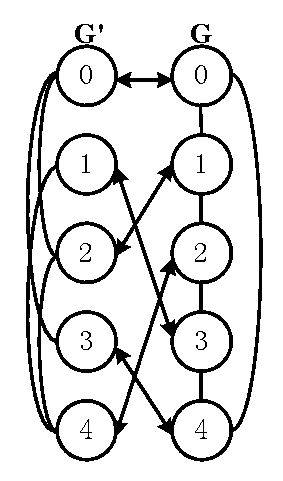
\includegraphics[width=.20\textwidth,height=.38\textwidth]{Visio-intercluster0.eps}
      \label{hfunction2}
    }
    \hspace{.5cm}
    \subfloat[集群间链路]{
      \includegraphics[height=.30\textwidth]{gg}
      %% 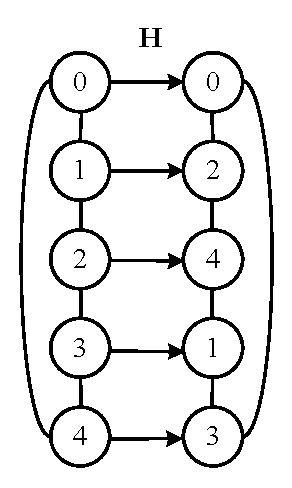
\includegraphics[width=.20\textwidth,height=.38\textwidth]{Visio-intercluster1.eps}
      \label{hfunction0}
    }
    \hspace{.5cm}
    \subfloat[完整结构]{
      \includegraphics[height=.30\textwidth]{edges}
      %% 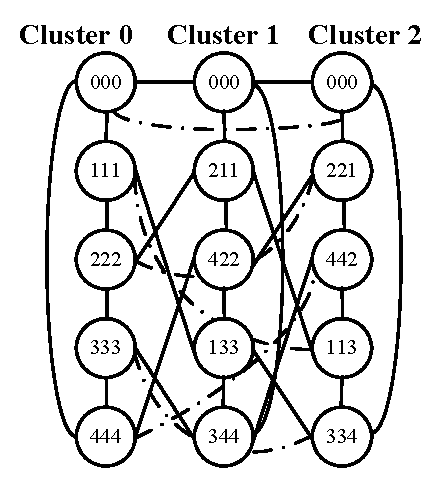
\includegraphics[width=.34\textwidth,height=.38\textwidth]{Visio-Hfunction1.eps}
      \label{hfunction1}
    }
    \caption{Galaxy图($n=3$,$q=5$)}
    \label{hfunction}
  \end{minipage}
\end{figure}

\subsubsection{Galaxy图网络直径}

关于Galaxy图的网络直径,有如下定理:
\begin{theorem}
\label{proofgalaxygraph}
Galaxy图的网络直径最多为2。
\end{theorem}

\begin{proof}

当$q=1$时,Galaxy图是一个全互连图,直径为1。

当$q>1$时,考虑Galaxy图中任意两个节点$n_i$、$n_j$,
它们的标号分别为$x_i$、$x_j$($x_i, x_j \in \mathds{F}_q$)。
可以分两种情况讨论:

(1)$n_i$、$n_j$属于同一个集群。
令$m = x_i - x_j$,如果$m \in X$ ,那么根据集群间链路构造规则,
在节点$n_i$与$n_j$之间存在一条链路,
$n_i$与$n_j$之间的最短路径长度为1。
如果$m \notin X$,$n_i$与$n_j$没有直接相连。
由于$n_i$与$n_j$都有$(q-\delta)/2$条链路连接
到同一集群内的其他节点,
那么从$n_i$与$n_j$出发,共有$q-\delta$条集群间链路
连接到其他$q-2$个节点。
因为$q-\delta > q-2$对于$\delta \in \{-1,0,1\}$恒成立,
所以节点$n_i$、$n_j$在集群内必定存在共同的邻节点,
此时$n_i$与$n_j$之间的最短路径长度为2。

(2)$n_i$、$n_j$属于不同的集群。
不失一般性地,假设$n_i \in V_s$,  $n_j \in V_t$,其中 $s < t$。
令$m = x_i - H(x_j) \bmod q$。
因为$m \in \mathds{F}_q$且$\mathds{F}_q = X \cup X' \cup \{0\}$,
又可以分为三种情况讨论:
(a) $m = 0$,此时由集群间链路构造规则可知,$n_i$与$n_j$之间存在一根链路,
$n_i$与$n_j$之间的最短路径长度为1。
(b) $m \in X$,那么集群$V_s$中标号为$H(x_j)$的节点
是$n_i$与$n_j$的共同邻节点,
此时$n_i$与$n_j$之间的最短路径长度为2。
(c) $m \in X'$,那么根据引理\ref{thm:isomorphic-function},
有$H^{-1}(x_i) - x_j \in X$,
也就是说,集群$V_t$中标号为$H^{-1}(x_i)$的节点
是$n_i$与$n_j$的共同邻节点,
此时$n_i$与$n_j$之间的最短路径长度为2。

综上所述,Galaxy图中任意一对节点之间最多2跳可达,即Galaxy图的直径为2。

\end{proof}

\subsection{拓扑构造}

%% Galaxyfly是一类低直径拓扑结构并由Galaxy图和全互连图组成。
%% 其使用端口数受限制的商用路由器也能满足可扩展性的需求。
%% Galaxyfly也是一个灵活的层次化结构,不仅可以较好
%% 的匹配高性能计算应用的通信模式特征,而且可以通过
%% 调整拓扑结构的参数配置和二分带宽以满足本地通信和
%% 全局通信。在表\ref{Table1}中介绍了Galaxyfly使用
%% 的参数表格。

将Galaxy图中的每一个节点替换成由$a$个路由器组成的超级节点,
超级节点内部$a$个路由器全互连,这样就得到了Galaxyfly拓扑结构。

Galaxyfly由5个基本参数$(n,q,a,p,h)$定义,表示为GF$(n,q,a,p,h)$。
表\ref{tab:gfparams}列出了这些基本参数的具体含义,
而表\ref{tab:gfderivedparams}列出了论文中使用到的其他符号的含义。
可以看出,GF$(n,q,a,p,h)$的基本结构如下:
整个网络由$n$个集群组成,
每个集群包含$q$个超级节点,
每个超级节点包含$a$个路由节点,
共计$N_r=nqa$个路由节点。
每个路由节点连接$p$个终端,
因此网络规模为$N=nqap$。

\begin{table}
  \centering
  \caption{Galaxyfly拓扑结构的基本参数}
  \label{tab:gfparams}
  \begin{tabular}{l l}
    \toprule
    参数 & 描述 \\
    \midrule
    $n$	& 网络中集群的数目\\
    $q$	& 单个集群中超级节点的数目\\
    $a$	& 单个超级节点中路由节点的数目\\
    $p$	& 单个路由节点连接终端的链路数目\\
    $h$ & 单个路由节点连接其他超级节点的链路数目\\
    \bottomrule
  \end{tabular}
\end{table}

\begin{table}
  \centering
  \caption{Galaxyfly拓扑结构的其他参数}
  \label{tab:gfderivedparams}
  \begin{tabular}{lll}
    \toprule
    参数 & 表达式   & 描述 \\
    \midrule
    $N_r$& $nqa$    & 网络中路由节点总数 \\
    $N$  & $nqap$   & 网络中终端总数(网络规模) \\
    $r$  &          & 路由器端口数\\
    $g$  & $a-1$    & 单个路由节点连接所在超级节点其他路由节点的链路数目\\
    $l_t$& $ap$     & 单个超级节点连接终端的链路数目\\
    $l_s$& $ah$     & 单个超级节点连接其他超级节点的链路数目\\
    $h_g$& $n-1$    & 单个超级节点连接其他集群超级节点的链路数目\\
    $h_s$& $(q-\delta)/2$ & 单个超级节点连接所在集群其他超级节点的链路数目\\
    \bottomrule
  \end{tabular}
\end{table}

具体到每个路由器,有$p$条链路连接到终端,
$g$条链路连接到同个超级节点内的其他路由器,
$h$条链路连接到其他超级节点内的路由器。
由于超级节点内部$a$个路由器全互连,因此$g=a-1$。
令$r$表示路由器的端口数,那么拓扑GF$(n,q,q,p,h)$
必须满足约束(\ref{gfcons0}),即路由器的链路总数不超过其端口数。

如果将超级节点看作一个虚拟结点,
那么该虚拟结点有$l_t=ap$条链路连接终端,$l_s=ah$条链路连接其他超级节点。
而根据Galaxy图的构造过程,$l_s$条连接其他超级节点的链路中,
至少要有$h_s=(q-\delta)/2$条链路通往所在集群其他超级节点与
$h_g=n-1$条链路通往其他集群的超级节点,共计$n-1+(q-\delta)/2$条链路,
因此由$l_s \ge h_g + h_s$我们得到GF$(n,q,q,p,h)$必须满足的另一个约束(\ref{gfcons1})。

\begin{equation}\label{gfcons0}
  r \ge p+(a-1)+h
\end{equation}
\begin{equation}\label{gfcons1}
  ah \ge n-1+(q-\delta)/2
\end{equation}

%% 一般情况,超级节点内部的链路和超级节点之间的链路分别是本地链路和全局链路。
%% 根据超级节点规模$a$的大小,我们可以设置集群内和集群之间的链路为本地链路
%% 和全局链路。超级节点和集群的概念类似于Dragonfly结构里超级节点和Slim Fly结构
%% 里子组的概念。

Galaxyfly拓扑中超级节点的概念与Dragonfly中的超级节点、Slim Fly中的子组相似。
层次化的网络结构使得Galaxyfly可以很好地适应不同HPC应用程序的流量特征。
通过调整参数$(n,q,a,p,h)$,
Galaxyfly可以在网络规模与二分带宽之间做灵活的折中
以适应不同种类的流量模式,如增大$a$以增加本地链路的比例适应以本地流量为主的应用。

\begin{table}
  \centering
  \caption{Galaxyfly参数配置示例}
  \label{tab:gfexample}
  \begin{tabular}{lcl}
    \toprule
    参数配置 & 网络直径 & 描述 \\
    \midrule
    GF$(n\!\!=\!\!1,q\!\!=\!\!1,a\!\!>\!\!1,p,h)$ & 1 & 全连通图\\
    GF$(n\!\!>\!\!1,q\!\!=\!\!1,a\!\!=\!\!1,p,h)$ & 1 & 全连通图\\
    GF$(n\!\!>\!\!1,q\!\!>\!\!1,a\!\!=\!\!1,p,h)$ & 2 & Galaxy图\\
    GF$(n\!\!>\!\!1,q\!\!=\!\!1,a\!\!>\!\!1,p,h)$ & 3 & Dragonfly结构\\
    GF$(n\!\!>\!\!1,q\!\!>\!\!1,a\!\!>\!\!1,p,h)$ & 5 & 通用Galaxyfly结构\\
    \bottomrule
  \end{tabular}
\end{table}

\paragraph{例}
Galaxyfly是一种高阶低直径的拓扑结构,
通过调整几个基本参数$(n,q,q,p,h)$可以搭建不同的互连网络。
表\ref{tab:gfexample}给出了一些例子。
其中GF$(n=1,q=1,a>1,p,h)$和GF$(n>1,q=1,a=1,p,h)$是全连通图,直径为1。
图\ref{largeGF0}展示了GF$(n>1,q>1,a=1,p,h)$的结构,
该配置实际就是Galaxy图,直径为2,它与Slim Fly类似,
可以看成一个扁平的网络,没有本地和全局的区别。
图\ref{largeGF1}展示了GF$(n>1,q=1,a>1,p,h)$的结构,
该配置本质上就是Dragonfly结构,即Dragonfly可以看作Galaxyfly的一个特例,其直径为3。
最后,GF$(n>1,q>1,a>1,p,h)$是通用Galaxyfly结构,直径为5,参见图\ref{largeGF2}。
事实上,Galaxyfly的网络直径上限为5。

\begin{figure}[t]
  \centering
    \begin{minipage}[t]{\textwidth}
   \centering
   \subfloat[GF($n>1,q>1,a=1,p,h$)]{
  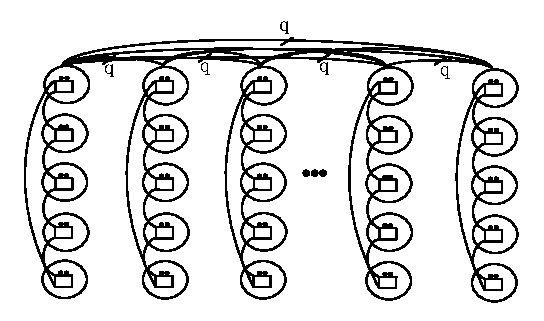
\includegraphics[width=.45\textwidth,height=.30\textwidth]{Visio-largeGF2.eps}
  \label{largeGF0}
  }
   \subfloat[GF($n>1,q=1,a>1,p,h$)]{
  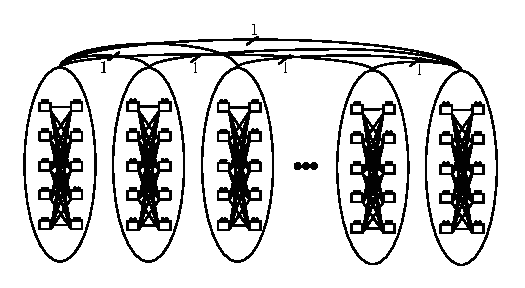
\includegraphics[width=.45\textwidth,height=.30\textwidth]{Visio-largeGF1.eps}
  \label{largeGF1}
  }

   \subfloat[GF($n>1,q>1,a>1,p,h$)]{
  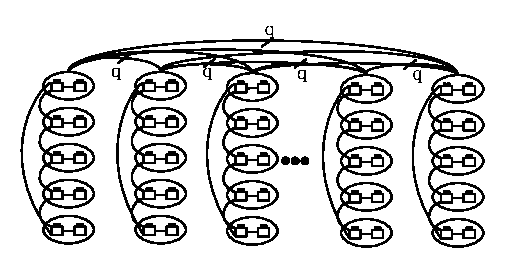
\includegraphics[width=.45\textwidth,height=.30\textwidth]{Visio-largeGF0.eps}
  \label{largeGF2}
  }
  \caption{Galaxyfly}
  \label{gfgraph}
    \end{minipage}
\end{figure}

\section{Galaxyfly结构分析}

在这一节中,我们分析Galaxyfly结构特征,包括灵活性,二分带宽,
最短路径和容错性。我们将Galaxyfly(GF)与其他典型拓扑结构,
如Dragonfly(DF)\upcite{dragonfly}、Flattened Butterfly(FB)\upcite{Flattenedbutterfly}、
Fat tree(FT)和Slim Fly(SF)\upcite{slimfly}进行对比分析。
在后续部分中,我们将使用缩写表示上述拓扑结构。

\subsection{灵活性}

灵活性是指一个拓扑结构构建不同规模的网络的能力,
一个灵活的拓扑结构允许通过调整参数支持构建从P级到E级甚至更大规模的高性能计算系统。
灵活性是一个高效的拓扑结构必须具备的属性。
在限定路由器端口数$r$的前提下,
我们通过比较不同拓扑支持搭建的网络规模范围来比较拓扑的灵活性。
%% 一种是使用一样端口数的路由器构造不同规模的网络。另一种则是使用不同端口数的路由器
%% 构造同一规模的网络。

通过调整参数$(n,q,a,p,h)$,GF可以用来搭建不同规模的互连网络。
使用48端口路由器,图\ref{fig:Figure4}描述了GF拓扑结构在不同参数配置下,
网络规模$N$与路由器连接终端数目$p$的关系。
在图\ref{fig:Figure4}中,我们选取了表\ref{tab:gfexample}中列出的配置,
其中网络直径为1、2、3的配置分别绘制在图\ref{fig:Figure40}、\ref{fig:Figure41}、\ref{fig:Figure42}中,
网络直径为5的配置绘制在图\ref{fig:Figure43}与\ref{fig:Figure44}中。
从图\ref{fig:Figure4}可以看出GF的规模可以从小于1K扩展至超过10000K。
其基本规律是,所选配置的网络直径越大,该配置可以支持的最大网络规模越大。
因此,GF其参数配置的实质是在网络规模和网络直径之间做折中。
最后,图\ref{fig:Figure43}和图\ref{fig:Figure44}展现了$a$的不同取值是如何影响网络规模的,
随着$a$的增大,可以构建的网络规模也随之增大。
%% FIXME
%% Q1: y labels in (b) and (c) are not consistent?
%% Q2: (d) and (e) use the same configuration?
%% REDRAW the figure.

\begin{figure}[t]
  \centering
  \begin{minipage}[t]{\textwidth}
   \centering
   \subfloat[GF$(n\!\!>\!\!1,q\!\!=\!\!1,a\!\!=\!\!1,p,h)$]{
  \includegraphics[width=.32\textwidth]{gfscale_a}
   \label{fig:Figure40}
  }
   \subfloat[GF$(n\!\!>\!\!1,q\!\!>\!\!1,a\!\!=\!\!1,p,h)$]{
  \includegraphics[width=.32\textwidth]{gfscale_b}
   \label{fig:Figure41}
  }
   \subfloat[GF$(n\!\!>\!\!1,q\!\!=\!\!1,a\!\!>\!\!1,p,h)$]{
  \includegraphics[width=.32\textwidth]{gfscale_c}
 \label{fig:Figure42}
  }\\
     \subfloat[ GF$(n\!\!>\!\!1,q\!\!=\!\!n,a\!\!>\!\!1,p,h)$]{
  \includegraphics[width=.32\textwidth]{gfscale_d}
 \label{fig:Figure43}
  }
     \subfloat[ GF$(n\!\!>\!\!1,q\!\!=\!\!n,a\!\!>\!\!1,p,h)$]{
  \includegraphics[width=.32\textwidth]{gfscale_e}
   \label{fig:Figure44}
  }

   \caption{不同配置下Galaxyfly的扩展性(使用48端口路由器)}
  \label{fig:Figure4}
  \end{minipage}
\end{figure}

图\ref{fig:Figure3}比较了GF与其他拓扑的灵活性。
其中,选取的FB与FT拓扑结构分别为3维FB与3层FT。
DF作为GF的一个特例,其本身可以通过调整参数$a$、$p$和$h$
来支持不同的网络规模,
但由于DF的最大规模以及均衡配置是在满足$a = 2p = 2h$的条件下取得,
因此在这里我们选取了该最佳配置。
对于GF,我们选取了$GF(n>1,q=n,a=2,p,h)$和$GF(n>1,q=n,a=3,p,h)$。
从图\ref{fig:Figure3}中可以看出,在给定端口数的条件下,
与其他拓扑结构相比,GF$(n>1,q=n,a=3,p,h)$可以构建出规模最大的互连网络,
同时可构建的网络规模范围也最大,即灵活性最高。
SF的优势在于,在指定节点度与严格限定网络直径为2的情况下,可以构建的网络规模最大,
然而,如果只限定路由器端口数,SF可以构造出的网络规模范围最小,灵活性最差。
尽管FT可以通过增加层数将规模扩展至100K,但需要使用大量的线缆与路由器,
成本开销过大且部署难度也会迅速提高。
DF是除GF外扩展性最佳的网络,优于FB与FT,
但在限定路由器端口为48的情况下,仍然无法搭建出100K的网络。

\begin{figure}[t]
  \centering
  \includegraphics[width=2.5in]{cmpscale}\\
  \caption{不同拓扑结构的扩展性(使用48端口路由器)}
  \label{fig:Figure3}
\end{figure}

%% 灵活性同时也表现在一个拓扑在同样规模下能用多少不同的路由端口数路由器构建。换句话说就是,不同的商用路由器能够被用来构造要求的网络规模。没有
%% 对路由器的限制。特别是GF结构,同一规模能够被不同的配置使用不同范围的
%% 端口数的路由器搭建网络。随着网络直径的增加,可构建要求规模的路由器端口数
%% 范围越大,而且在大部分情况下支持的最小端口数则越低。

\subsection{二分带宽}
一般地,在设计互连网络时要给定目标网络的规模$\bar{N}$。
对Galaxyfly而言,选取的参数$(n,q,a,p,h)$必须使得网络规模达到目标规模,
如式(\ref{gfcons2})所示。
\begin{equation}\label{gfcons2}
  nqap \ge \bar{N}
\end{equation}

可行配置不仅要网络规模的要求,还要满足二分带宽的要求。
二分带宽是所有网络平均二分中最小切割的带宽,是评价拓扑结构性能的传统指标。
我们假设每条链路的带宽为1,那么网络的最小二分切割$C_{min}$就等于二分带宽。
在均衡随机通信负载下,只要图的二分最小切割有$N/4$条双向链路就使网络是均衡负载的,
于是我们得到Galaxyfly设计的一个性能约束,$C_{min} \ge N/4$。
由于非堵塞拓扑结构要求至少有$N/2$条双向链路通过图的最小二分切割,
令$\beta=C_{min}/(N/2)$,那么$C_{min} \ge N/4$可以等价地表示为式(\ref{gfcons3})。
\begin{equation}\label{gfcons3}
  \beta \ge 0.5
\end{equation}

至此,我们得到了Galaxyfly的可行参数配置空间,
该空间为约束(\ref{gfcons0})--(\ref{gfcons3})构成的集合。

令端口数上限$r \le 48$(当前商用高阶路由器端口数),
图\ref{chap03figure6}展示了在可行参数配置空间中找到的
$\beta \approx 0.5$的Galaxyfly配置的网络规模。
我们选取SF、3D FB、5D FB作为对比,将他们的网络规模也绘制在图\ref{chap03figure6}中。
由于GF和SF的不规则性,这两种拓扑结构的二分带宽无简单的解析表示。
因此对于GF和SF,我们使用图划分工具METIS\upcite{METIS}近似求解它们的二分带宽。
我们按照网络直径分组,同一张图中展示出的拓扑机构具有相同的网络直径。

\begin{figure}[t]
  \centering
  \begin{minipage}[t]{\textwidth}
    \centering
    \subfloat[网络直径$D=2$]{
      \includegraphics[width=.4\textwidth]{bbw_sf_a}
      %% 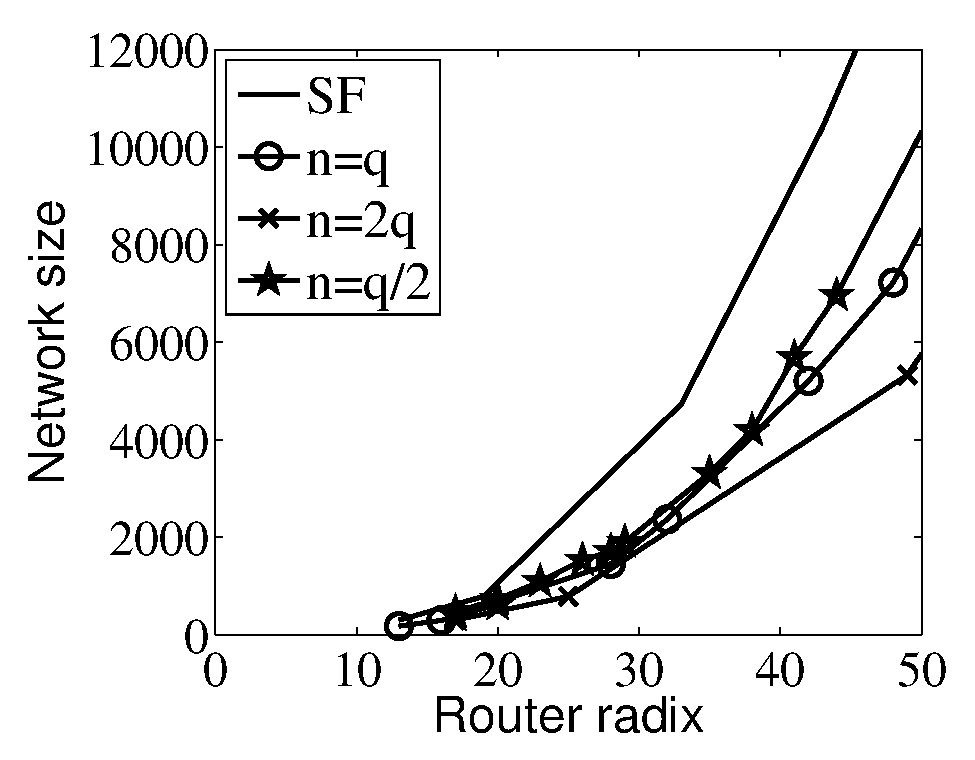
\includegraphics[width=.4\textwidth]{BB_1_v11.eps}
      \label{fig:bbw_sf_a}
    }
    \subfloat[网络直径$D=2$]{
      \includegraphics[width=.4\textwidth]{bbw_sf_b}
      %% 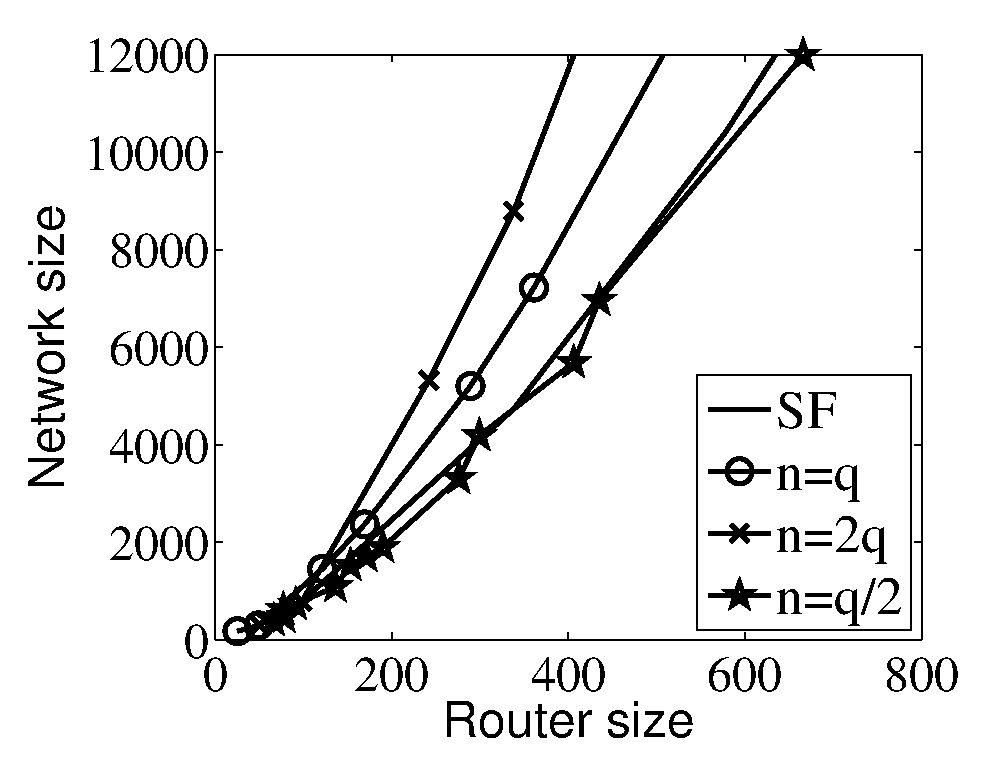
\includegraphics[width=.4\textwidth]{BB_1_v12.eps}
      \label{fig:bbw_sf_b}
    }
    \\
    \subfloat[网络直径$D=3$]{
      \includegraphics[width=.4\textwidth]{bbw_3dfb_a}
      %% 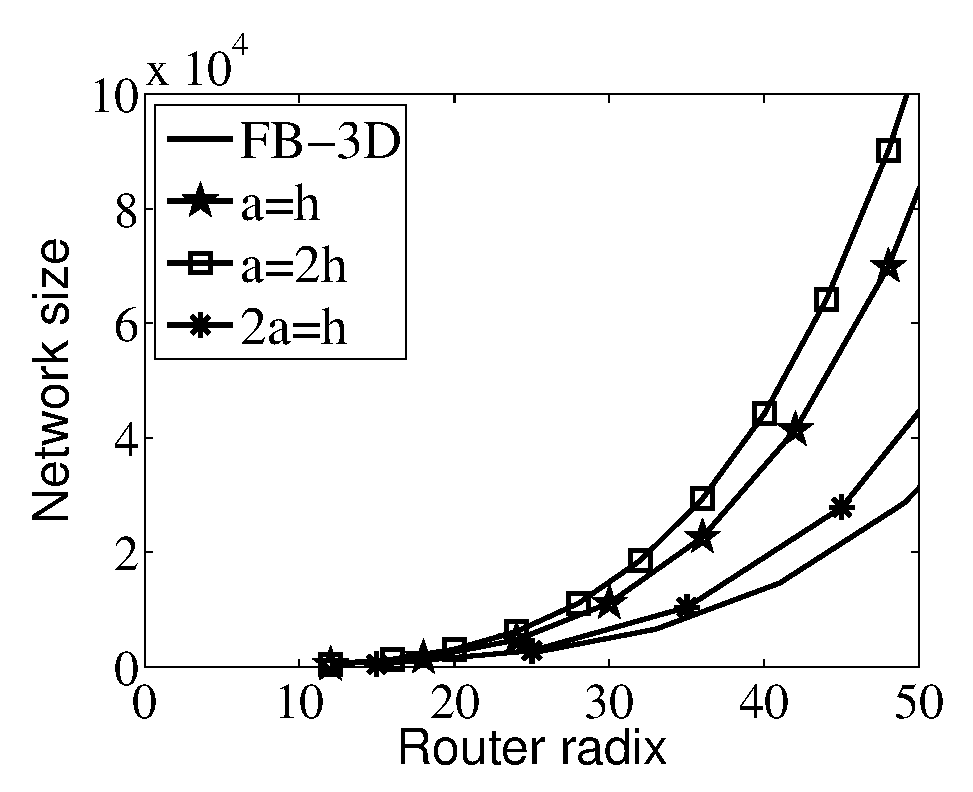
\includegraphics[width=.4\textwidth]{BB_1_v13.eps}
      \label{fig:bbw_3dfb_a}
    }
    \subfloat[网络直径$D=3$]{
      \includegraphics[width=.4\textwidth]{bbw_3dfb_b}
      %% 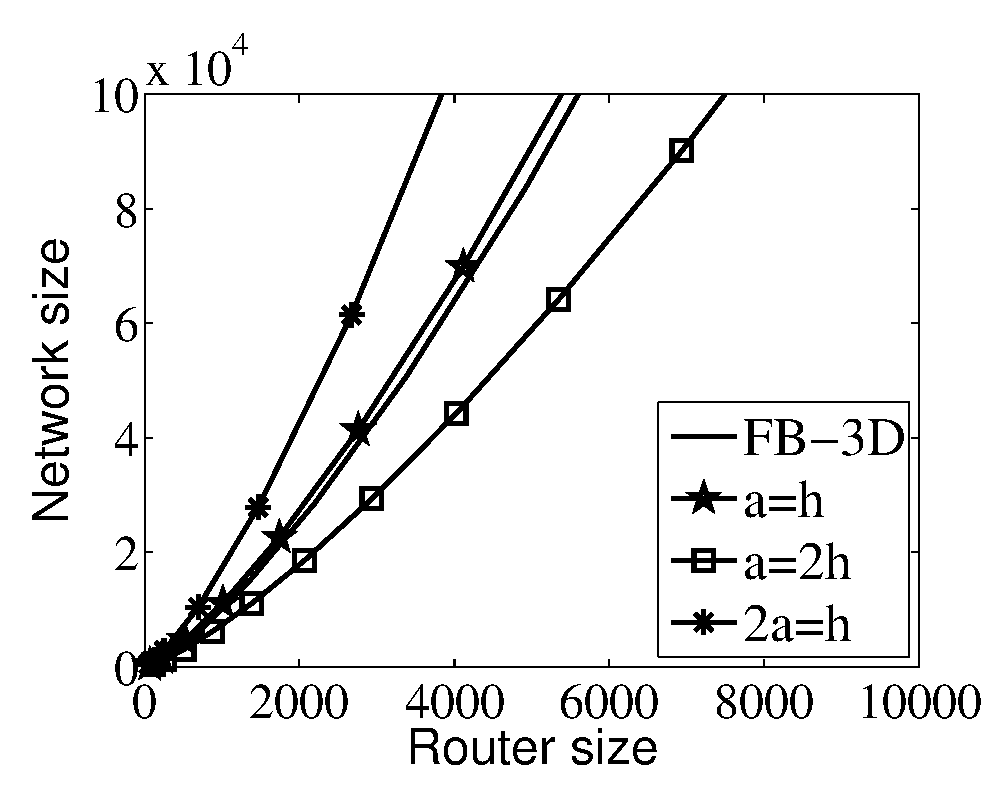
\includegraphics[width=.4\textwidth]{BB_1_v14.eps}
      \label{fig:bbw_3dfb_b}
    }
    \\
    \subfloat[网络直径$D=5$]{
      \includegraphics[width=.4\textwidth]{bbw_5dfb_a}
      %% 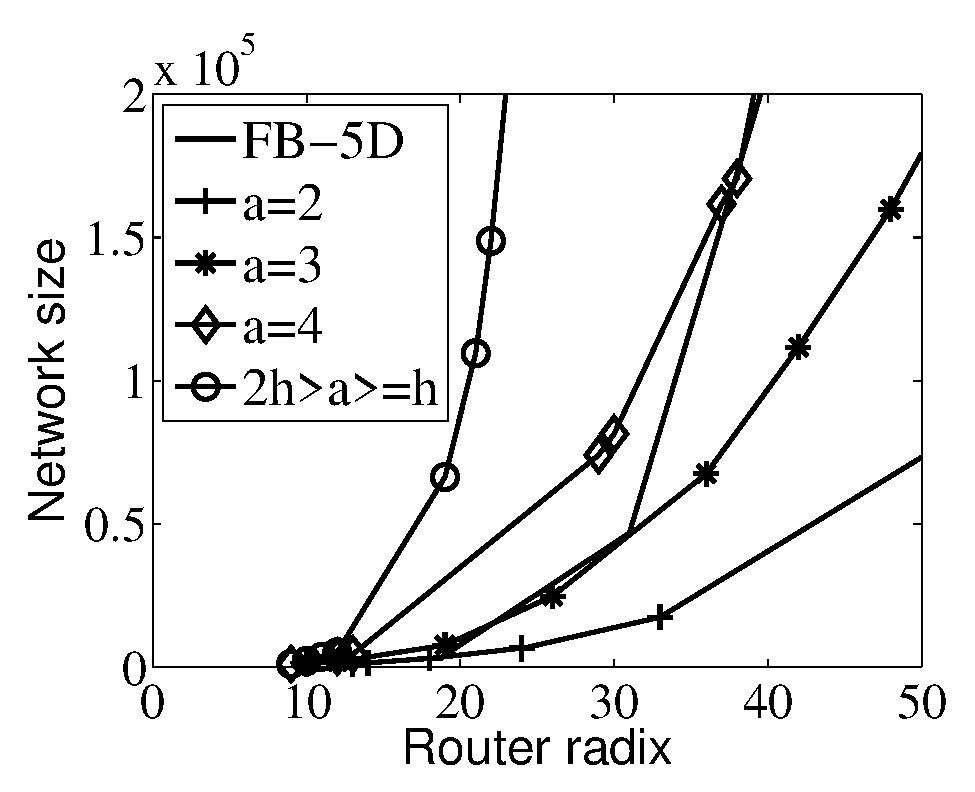
\includegraphics[width=.4\textwidth]{BB_1_v15.eps}
      \label{fig:bbw_5dfb_a}
    }
    \subfloat[网络直径$D=5$]{
      \includegraphics[width=.4\textwidth]{bbw_5dfb_b}
      %% 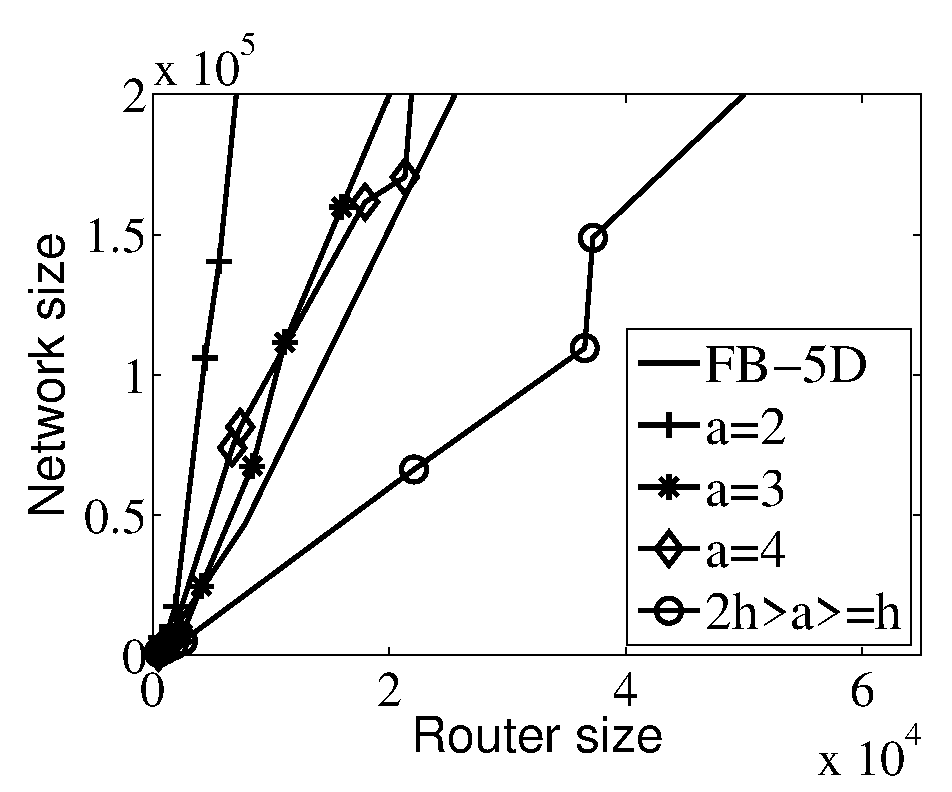
\includegraphics[width=.4\textwidth]{BB_1_v16.eps}
      \label{fig:bbw_5dfb_b}
    }
    \caption{Galaxyfly在$\beta \approx 0.5$时的网络规模与路由器总数}
    \label{chap03figure6}
  \end{minipage}
\end{figure}

图\ref{fig:bbw_sf_a}、图\ref{fig:bbw_3dfb_a}和图\ref{fig:bbw_5dfb_a}
描述了随着端口数$r$增加,网络规模$N$的变化趋势。
相应地,图\ref{fig:bbw_sf_b}、图\ref{fig:bbw_3dfb_b}和图\ref{fig:bbw_5dfb_b}
描述了随着网络规模$N$的增加,路由器数量$N_r$的增长趋势。
图\ref{fig:bbw_sf_a}与图\ref{fig:bbw_sf_b}展示了直径为2的网络SF与GF$(n,q,a=1,p,h)$。
对于GF,我们选择了三种不同的$n$和$q$的比例。
由图可知,使用同样的路由器端口数$r$,SF可以构造最大规模的直径为2的网络,
但是,在同一规模下,GF$(n=q,q,a=1,p,h)$和GF$(n=2q,q,a=1,p,h)$
使用的路由器数量比SF更少。
图\ref{fig:bbw_3dfb_a}与图\ref{fig:bbw_3dfb_b}展示了直径为3的网络3D FB与GF$(n,q=q,a,p,h)$。
这里的GF$(n,q=1,a,p,h)$本质上就是DF结构。
我们选择了三种不同的$a$和$h$的比例。
当$a=2h$时(此时$n=a^{2}/2+1$),GF$(n,q=1,a,p,h)$网络均衡且规模最大,
它比3D FB结构的扩展性好。
但是,在限定路由器端口数为48时,其最大规模仍然不能达到100K。
图\ref{fig:bbw_5dfb_a}与图\ref{fig:bbw_5dfb_b}展示了直径为5的网络5D FB与GF$(n=q,q,a,p,h)$。
对于GF的参数$a$,我们选择了四种不同的值。
由图可知,5D FB、GF$(n=q,q,a=4,p,h)$与GF$(n=q,q,h\leq{}a<2h,p,h)$在使用48端口的路由器时
可以构造100K规模的网络。
其中,GF$(n=q,q,h\leq{}a<2h,p,h)$使用路由器最多,
但是,它需要的路由器的端口数是最小。
在网络规模为200K 时,GF$(n=q,q,h\leq{}a<2h,p,h)$需要的路由器端口数仅为5D FB的一半。

我们还分析了不同$\beta$下,路由器数量和网络规模的关系。
表\ref{chap3table5}列出了一些GF和DF实例的$\beta$、路由器数量$N_r$与网络规模$N$,
这些GF与DF实例采用相同的配置$a=2h=2p$。
从表中可以看出,$\beta$的值越高,则需要更多的路由搭建同一规模的网络。
GF的规模可以达到接近$a^2/4$倍DF的规模,而其其二分带宽只是稍微低于DF。
因此,在满足给定二分带宽需求的前提下,GF可以使用同样的路由器构造更大规模的网络。

%% FIXME 表里的r是多少?为什么不把N也列出来?
\begin{table}[t]
\caption{同样参数配置$a$、$h$和$p$的Galaxyfly和Dragonfly的二分带宽}
\centering
\begin{tabular}{ccccc}
  \toprule
  Topology & GF$(n,q,a,p,h)$ & $N_r$ & \tabincell{c}{二分带宽}	& $\beta$\\
  \midrule
  \multirow{5}*{DF}
  &$GF(9,1,4,2)$	&36	&20	&0.56 \\
  &$GF(19,1,6,3)$	&114	&94	&0.55 \\
  &$GF(33,1,8,4)$	&264	&275	&0.52 \\
  &$GF(55,1,10,5)$	&550	&701	&0.51 \\
  &$GF(73,1,12,6)$	&876	&1332	&0.51 \\
  \midrule
  \multirow{5}*{GF}
  &$GF(5,7,4,2)$	&140	&44	&0.31	\\
  &$GF(9,19,6,3)$	&1026	&560	&0.36 \\
  &$GF(17,31,8,4)$	&4216	&2350	&0.28 \\
  &$GF(30,53,10,5)$	&15900	&14026	&0.35 \\
  &$GF(37,73,12,6)$	&32412	&36676	&0.38 \\
  \bottomrule
\end{tabular}
 \label{chap3table5}
\end{table}

二分带宽是一个理论指标,是网络平均二分之间的带宽上限,
给定不同通信模式和不同路由算法,有效的二分带宽小于理论的二分带宽\upcite{multistage}。
%% FIXME 这一句到底想表达什么呢!!!!!!!!!!!!!
另外,在GF的超级节点采用的全互连图中,二分带宽为$a^2/4$。
如果超级节点不堵塞,那么要求在均衡随机通信模式下,至少需要$ap/2$条双向链路。
如果我们设计一个可行的GF配置,也不得不考虑超级节点内的参数配置。

\subsection{最短路径}

最短路径数量是一个负载均衡的网络重要的指标。表\ref{Tablesp}
列出了不同配置下的GF与SF的最短路径数量。$SP$是指最短路径数量大于1
的节点对数量与网络中所有节点对总数$N_r(N_r-1)/2$的比值。
集群内$SP$是指集群内最短路径数大于1的节点对数量与网络中所有节点对总量的比值,
对应地,集群间$SP$指集群间最短路径数大于1的节点对数量与网络中所有节点对总数的比值。
对于SF,尽管在限定网络直径为2的情况下可以构造最大规模的网络,
但是其最短路径数量却远远小于表中列出的GF配置。
GF$(n>1,q>1,a=1,p,h)$也是一个直径为2的拓扑结构,
与SF相比,它的SP更高,但用于连接其他路由器的端口数$h+a-1$也更大,
这使得GF$(n>1,q>1,a=1,p,h)$拥有多于SF的链路数量。
GF$(n>1,q=1,a>1,p,h)$是DF结构,它的$SP$值略大于GF$(n<1,q>1,a=1,p,h)$的SP,
且使用了更少的端口数,但集群内的最短路径数少。
GF$(n>1,q>1,a>1,p,h)$的SP最高而且使用的路由器端口数最少,
然而它的网络直径是5,是表中列出的网络中直径最大的一个。绝大多数集群内
$SP$是低于集群间$SP$的,因此,为了提高网络的负载均衡,
应该尽量充分利用集群间的最短路径数量。

\begin{table}[t]
\caption{Galaxyfly与Slim Fly的最短路径数量}
\centering
\begin{tabular}{cccccc}
  \toprule
  拓扑结构 & $h+a-1$ & $N_r$ & $SP$ & 集群内$SP$ & 集群间$SP$\\
  \midrule
  \multirow{2}*{$SF$}
  &25		&578	 &0.01 &0.01 & 0 \\ %\cline{2-6}
  &35		&1058	 &0.05 &0.01 & 0.04\\
  \midrule
  \multirow{2}*{$GF(n\!\!>\!\!1,q\!\!>\!\!1,a\!\!=\!\!1,p,h)$}
  &31		&496	&0.14 &0.03 &0.11\\
  &47		&992	&0.13 &0.01 &0.12\\
  \midrule
  \multirow{2}*{$GF(n\!\!>\!\!1,q\!\!=\!\!1,a\!\!>\!\!1,p,h)$}
  &14		&510	&0.17 &0 &0.17\\
  &17		&876	&0.15 &0 &0.15\\
  \midrule
  \multirow{2}*{$GF(n\!\!>\!\!1,q\!\!>\!\!1,a\!\!>\!\!1,p,h)$}
  &8		&510	&0.43 &0.03 &0.41\\
  &8		&966	&0.51 &0.06 &0.44\\
  \bottomrule
\end{tabular}
\label{Tablesp}
\end{table}

\subsection{容错性}

我们通过模拟随机链路的出错来分析拓扑结构的容错性。
采用的具体方法是,逐渐提升网络链路随机出错的概率直至网络不连通,
观察网络的平均路径长度与网络直径如何随链路出错率变化而变化。
图\ref{fig:Figure8a}与图\ref{fig:Figure8b}
分别展示了不同配置下的GF和其他拓扑结构的平均最短路径和网络直径
随着链路出错率增加而变化的情况。
图\ref{nr1}和图\ref{nr2}展示了GF$(n>1,q>1,a=1,p,h)$和SF在路由器
规模在0.2K-2K范围内容错性的变化情况。
图\ref{nr3}和图\ref{nr4}展示了GF$(n>1,q>1,a>1,p,h)$和DF在路由器
规模在0.2K-2K范围内容错性的变化情况。
对于GF、DF和SF,容错性随着路由器规模的增加而提升。
在路由器规模为2K的情况下,GF$(n>1,q>1,a=1,p,h)$可以容忍$90\%$的链路出错率,
而SF的链路错误容忍度为$86\%$。
GF$(n>1,q>1,a>1,p,h)$和DF分别只能容忍$60\%$和$65\%$的链路出错率。
GF$(n>1,q>1,a=1,p,h)$和SF的容错性能比GF$(n>1,q>1,a>1,p,h)$和DF
在同一规模下容错性好是因为更短的网络直径和更多的链路。

\begin{figure}
  \centering
  \begin{minipage}[t]{\textwidth}
    \centering
    \subfloat[平均路径长度]{
      \includegraphics[width=.4\textwidth]{resiliency_a}
      \label{nr1}
    }
    \subfloat[网络直径]{
      \includegraphics[width=.4\textwidth]{resiliency_b}
      \label{nr2}
    }
    \caption{$GF(n\!\!>\!\!1,q\!\!>\!\!1,a\!\!=\!\!1,p,h)$与SF的容错性}
  \label{fig:Figure8a}
  \end{minipage}
\end{figure}
\begin{figure}
  \centering
  \begin{minipage}[t]{\textwidth}
    \centering
    \subfloat[平均路径长度]{
      \includegraphics[width=.4\textwidth]{resiliency_c}
      \label{nr3}
    }
    \subfloat[网络直径]{
      \includegraphics[width=.4\textwidth]{resiliency_d}
      \label{nr4}
    }
    \caption{$GF(n\!\!>\!\!1,q\!\!>\!\!1,a\!\!>\!\!1,p,h)$与DF的容错性}
    \label{fig:Figure8b}
  \end{minipage}
\end{figure}


\section{路由算法}

本节将给出Galaxyfly结构的最短路径路由算法与非最短自适应路由算法,
并介绍与路由算法配套的死锁避免机制。在本节路由算法的讨论中,
假设报文从源节点直接传输给直接相连的源路由节点$R_s$并由此路由至与目的节
点直接相连的目的路由节点$R_d$。

\subsection{最短路径路由算法}

%% 由于Galaxyfly是将Galaxy图中的节点代之以$a$个路由器全互连组成的超级节点得到
%% 的层次化互连网络,因此Galaxyfly网络的最短路由算法中最段路径的计算
%% 可以分层进行。即,先寻找超级节点$G_s$与$G_d$之间的最短路径,
%% 在此基础上计算路由节点$R_s$与$R_d$之间的最短路径。

%% 上述思路不正确
%% 路由节点间的最短路径并不一定通过所在超级节点间的最短路径

\begin{algorithm}[t]
  \caption{Galaxyfly网络最短路径算法}
  \label{alg:min}
  \algsetup{indent=1em}
  \begin{algorithmic}[1]
    \REQUIRE 源路由节点$R_s$
    \ENSURE $R_s$到所有其他路由节点$R_d$的最短路径集合$P_{s,d}$,
    %% $\P_{s,d} = \{P_{s,d}^0, P_{s,d}^1, \cdots, P_{s,d}^{K_{s,d}-1}\}$,\\
    其中$d \in [0, N_r)$且$d \neq s$
    \STATE $P_{s,s} \gets \lbrace [R_s] \rbrace$ \label{l:res.init.self}
    \FOR {$d \in [0, N_r) \land d \neq s$} \label{l:res.init.begin}
    \STATE $P_{s,d} \gets \emptyset$
    \ENDFOR \label{l:res.init.end}
    \STATE $V \gets \lbrace R_s \rbrace$ \label{l:v}
    \STATE $Q_c \gets \lbrace R_s \rbrace$ \label{l:qc}
    \STATE $Q_n \gets \emptyset$ \label{l:qn}
    \WHILE {$Q_c \neq \emptyset$} \label{l:bfs.begin}
    \FOR {$R \in Q_c$} \label{l:expand.begin}
    \STATE $Q_n \gets Q_n \bigcup (neighbors(R) - V)$
    \ENDFOR \label{l:expand.end}
    \FOR {$R_d \in Q_n$} \label{l:rd}
    \FOR {$R_x \in neighbors(R_d) \bigcap V$} \label{l:rx}
    \STATE $P_{s,d} = \lbrace\ append(p, R_d)\ |\ \forall p \in P_{s,x}\ \rbrace$ \label{l:psd}
    \ENDFOR
    \ENDFOR
    \STATE $Q_c \gets Q_n$ \label{l:qc.update}
    \STATE $Q_n \gets \emptyset$ \label{l:qn.update}
    \ENDWHILE \label{l:bfs.end}
  \end{algorithmic}
\end{algorithm}

Galaxyfly网络中节点间最短路径可能不唯一,
在报文从源路由节点$R_s$向目的路由节点$R_d$的传输过程中,
应尽量均衡地利用多个最短路径以平衡网络负载。
因此,最短路径路由算法应记录任意节点对$R_s$、$R_d$之间的所有最短路径。
算法\ref{alg:min}给出了计算Galaxyfly网络中给定源路由节点$R_s$到
其他所有路由节点的最短路径集合的算法。
Galaxyfly是一个无向、无环、连通图,
算法\ref{alg:min}是一个基于宽度优先搜索(BFS)的遍历算法,
在搜索过程中完成$R_s$到任意节点$R_d$最短路径集合$P_{s,d}$的计算。
首先,$R_s$到自身的最短路径初始化为$\{[R_s]\}$(第\ref{l:res.init.self}行),
$R_s$到所有其他路由节点$R_d$的最短路径集合初始化为空集
(第\ref{l:res.init.begin}--\ref{l:res.init.end}行)。
之后,建立三个辅助数据结构$V$,$Q_c$,$Q_n$,
其中$V$表示已经访问过的节点集合(第\ref{l:v}行),
$Q_c$与$Q_n$分别表示BFS过程中当前正在扩展的节点集合与
下一次将要扩展的结点集合(第\ref{l:qc}--\ref{l:qn}行)。
算法的主循环(第\ref{l:bfs.begin}--\ref{l:bfs.end}行)执行BFS过程。
在BFS过程的每一次迭代中,
首先将$Q_c$中每个路由节点$R$的未访问过的邻居节点加入$Q_n$
(第\ref{l:expand.begin}--\ref{l:expand.end}行)。
然后,对$Q_n$中每一个路由节点$R_d$(第\ref{l:rd}行),
开始计算$R_s$到$R_d$的最短路径集合$P_{s,d}$,
具体方法如下:对于$R_d$的邻居节点$R_x$,如果$R_x \in V$,即$R_x$已经访问过(第\ref{l:rx}行),
那么将$R_d$添加到从$R_s$到$R_x$的任意最短路径$p$尾部即可得到一条
从$R_s$到$R_d$的最短路径(第\ref{l:psd}行)。
最后,更新扩展队列集合$Q_c$与$Q_n$(第\ref{l:qc.update}--\ref{l:qn.update}行)。

%% \begin{algorithm}[t]
%%   \caption{Galaxyfly网络最短路径算法}
%%   \label{alg:min}
%%   \algsetup{indent=1em}
%%   \begin{algorithmic}[1]
%%     \REQUIRE 源路由节点$R_s$,目标路由节点$R_d$
%%     \ENSURE $R_s$到$R_d$的最短路径集合$P_{min} = \{P_0, P_1, \cdots, P_{K-1}\}$,其中\\
%%     $P_k=[R_k^0, R_k^1, \cdots, R_k^{n-1}]$,$k \in [0, K)$为$R_s$到$R_d$的一条长度为$n$的最短路径
%%     \STATE $P_{min} \gets \emptyset$
%%     \STATE $G_s \gets supernode(R_s)$
%%     \STATE $G_d \gets supernode(R_d)$
%%     \IF {$G_s = G_d$}
%%     \STATE $P_{min} \gets \{[R_s, R_d]\}$
%%     \ELSIF {connected($G_s$, $G_d$)}
%%     \STATE $S \gets \{\ R_x\ |\ \forall (R_x, R_y) \in edges(G_s, G_d)\ \}$
%%     \STATE $D \gets \{\ R_y\ |\ \forall (R_x, R_y) \in edges(G_s, G_d)\ \}$
%%     \IF {$R_s \in S \land R_d \in D$}
%%     \STATE $P_{min} \gets \{\ [R_s, R_d]\ \}$
%%     \ELSIF {$R_s \in S \land R_d \notin D$}
%%     \STATE $P_{min} \gets \{\ [R_s, R_y, R_d]\ |\ \forall R_y \in D \land (R_s, R_y) \in edges(G_s, G_d)\ \}$
%%     \ELSIF {$R_s \notin S \land R_d \in D$}
%%     \STATE $P_{min} \gets \{\ [R_s, R_x, R_d]\ |\ \forall R_x \in S \land (R_x, R_d) \in edges(G_s, G_d)\ \}$
%%     \ELSIF {$R_s \notin S \land R_d \notin D$}
%%     \STATE $P_{min} \gets \{\ [R_s, R_x, R_y, R_d]\ |\ \forall (R_x, R_y) \in edges(G_s, G_d)\ \}$
%%     \ENDIF
%%     \ELSE
%%     \STATE $GG \gets \{\ G_m\ |\ connected(G_s, G_m) \land connected(G_m, G_d)\ \}$
%%     \FOR {$G_m \in GG$}
%%     \STATE $t_m \gets 5$
%%     \STATE $S \gets \{\ R_x\ |\ \forall (R_x, R_y) \in edges(G_s, G_m)\ \}$
%%     \STATE $M_S \gets \{\ R_y\ |\ \forall (R_x, R_y) \in edges(G_s, G_m)\ \}$
%%     \STATE $M_D \gets \{\ R_x\ |\ \forall (R_x, R_y) \in edges(G_m, G_d)\ \}$
%%     \STATE $D \gets \{\ R_y\ |\ \forall (R_x, R_y) \in edges(G_m, G_d)\ \}$
%%     \IF {$R_s \in S$}
%%     \STATE $t_m \gets t_m - 1$
%%     \ENDIF
%%     \ENDFOR
%%     \ENDIF
%%   \end{algorithmic}
%% \end{algorithm}

为得到Galaxyfly网络中所有节点对之间的最短路径,
只需对所有路由节点运行一次算法\ref{alg:min}即可。
完成所有路由节点对的最短路径计算后,
可以通过配置路由表等方式实现最短路由算法MIN,
在路径选择方面可以使用简单的令牌方式均衡使用不同的最短路径。

\subsection{非最短路径自适应路由算法}

我们为Galaxyfly设计了三种非最短自适应路由算法,分别是
非最短自适应随机链路路由算法(NAR),
非最短自适应本地链路路由算法(NAL),以及
非最短自适应全局链路路由算法(NAG),
他们都是基于Galaxyfly结构特性、非最短路径路由算法以及全局
自适应负载均衡路由算法设计的\upcite{Singh}\upcite{slimfly}\upcite{dragonfly}。
为了控制两个终端的之间的跳步数和减少虚拟通道(VC)的数量,非最短
自适应路径会限制随机选择路径的长度。
%% 使得最长路径分别在5跳、6跳或者7跳以内。
NAR使用的策略是,只有当两个终端处于同一个集群的两个不同的超级节点时,
才会执行非最短路由。该策略的目的是限制非最短路由的路径长度,
使得非最短路径长度最多为6跳。
%% FIXME 这句话在说什么?
%% 因为,两个超级节点之间可能存在多个公共相邻超级节点。
NAL的策略是是允许在源超级节点内多绕行1跳,其非最短路径的长度限制为6跳。
NAG的策率则是允许绕行到别的超级节点,其非最短路径的长度限制为7跳,
(3跳超级节点间链路与4跳超级节点内的链路)。
%% 因此,在NAL与NAR中,非最短路径的长度限制分别为6跳和7跳。
%% FIXME 那么NAR是5跳?

非最短路径自适应路由主要用于最短路径过载的情况下。
网络负载状态的判定在路由器本地完成,
主要依据为当前路由器的缓冲区状态。
%% FIXME 这对应三种算法?为什么有三个?
具体来说,是根据缓冲区队列的占有率来选择使用最短路径路由或是非最短路径自适应路由。
令$Q_{min}$与$Q_{nonmin}$分别表示最短路径端口与非最短路径端口的缓冲区队列的占有率,
$Th_{min}$和$Th_{nonmin}$分别表示选择走最短路径和非最短路径的阈值。
若$Q_{min}>Th_{min}$且$Q_{nonmin}<Th_{nonmin}$,那么报文将通过非最短路径传输。
$Th_{nonmin}$和$Th_{min}$是经验参数,可以通过模拟进行调优。
%% 在我们的实验中,这两个阈值分别被设置为
%% $Th_{nonmin}=0.5Q_{min}$ 和 $Th_{min}=0.8\times$ $缓冲区容量$。

\subsection{死锁避免机制}

Galaxyfly的死锁避免机制与Dragonfly\upcite{dragonfly}和
Slim Fly\upcite{slimfly}的死锁避免机制类似。
基于距离的死锁避免机制每一跳都切换一条VC,
因此,需要的VC数量与最长路径跳步数相同。
在Galaxyfly结构中,我们使用递增的方法分配VC。
即,报文开始注入时使用编号为0的VC,每经过一跳使用的
VC编号加一\upcite{Prevention}\upcite{Rlmolm}。
报文在最后一条VC的时候不会被堵塞是因为报文要被吸收。
因此,报文要么前进走更高编号的VC,要么就是要被终端吸收。
由于Galaxyfly划分了超级节点,我们能复用本地端口的VC和全局端口的VC,
这样可以减少VC的数量。

图\ref{fig:Figure9}说明了不同网络直径的Galaxyfly网络中
最短路径路由是如何使用VC的避免死锁的。
例如,在图\ref{fig:Figure93}所示的最短路径路由中,
报文最多经过3条本地链路和2条全局链路。
因此,在MIN中要求至少3条本地链路VC和2条全局链路VC来避免出现环。
%% FIXME 不是又复用?按图上的表示应该是3条VC就够了呀
类似地,NAR、NAL以及NAG算法分别需要3、4、4条本地链路VC和2、2、3条全局链路VC。

除上述依赖VC的死锁避免机制以外,Galaxyfly也可以使用逃逸网络或者转弯模型方法来避免死锁
\upcite{Rlmolm}\upcite{OFAR-CM}\upcite{On-the-Fly}。

\begin{figure}[t]
  \centering
   \begin{minipage}[t]{\textwidth}
   \centering
  \subfloat[网络直径$D=2$]{
  \includegraphics[width=.25\textwidth]{Visiomind1.eps}
  \label{fig:Figure91}
  }
  \subfloat[网络直径$D=3$]{
  \includegraphics[width=.5\textwidth]{Visiomind2.eps}
  \label{fig:Figure92}
  }
  \\
  \subfloat[网络直径$D=5$]{
  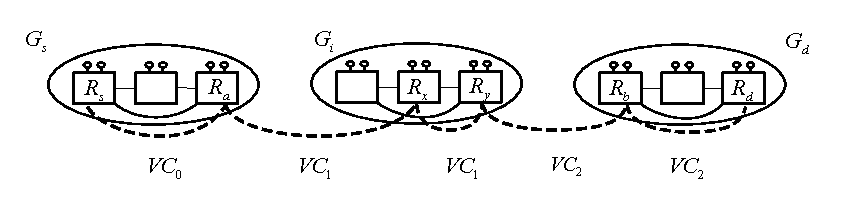
\includegraphics[width=.75\textwidth]{Visiomind3.eps}
  \label{fig:Figure93}
  }
  \caption{Galaxyfly最短路径路由算法中的VC使用}
  \label{fig:Figure9}
  \end{minipage}
\end{figure}

\section{性能分析}

在这一章节中,我们使用一个时钟精确的网络模拟器Booksim\upcite{Booksim}模拟Galaxyfly
和其他拓扑结构的运行来分析比较不同拓扑结构的性能。
实验采用伯努力分布报文注入模型。
首先,我们在几种典型的通信模式下评测了不同配置下的Galaxyfly网络,
分析了在不同的报文长度及不同路由算法下的网络性能。
第二,我们比较了Galaxyfly和其他高阶拓扑结构在不同的通信模式下的性能,
包括一种新的混合通信模式。
第三,我们在物理布局对网络延迟产生影响的情况下评测了不同拓扑结构的性能。

\subsection{实验设置}

\subsubsection{路由器}

我们使用传统的具备完整的路由器流水线的输入队列(Input Queue,IQ)路由器模型。
路由器基于Virtual Cut-through(VCT)交换机制。
我们假设信用处理过程需要2个时钟周期,路由计算模块需要2个时钟周期,
交换分配模块、虚通道(VC)分配模块和crossbar处理模块都需要1个时钟周期,
crossbar的输入和输出的加速比都是1,内部传输数据链路速率是链路传输速率的两倍。
路由器每个输入端口的缓冲区容量是256个切片。
缓冲区的管理机制采用每个VC拥有5个切片的私有存储空间,
其他的缓冲区由所有VC共享。

\subsubsection{网络类型}
%% 默认情况下,链路传输延迟为1个时钟周期,报文长度为1个切片大小。
我们提供了两种链路传输延迟配置。
一种是每一条链路的传输延迟都是1个时钟周期。
%% FIXME 下面这句啥意思?
在这种配置下,我们可以减少不同拓扑结构在构造同等规模的网络时
使用不同端口数的路由器而造成的影响并观察网络状态。
在文献\upcite{slimfly}与文献\upcite{dragonfly}中,
链路传输延迟即采用这种配置。
第二种配置是根据物理布局中的位置设置延迟,
其目的是为了模拟实际系统物理布局对延迟造成的影响。
机柜间链路包括路由器流水线的延迟一共100个周期,
而机柜内链路则是50个周期。

表\ref{chap3table6}列出了实验中选用的所有拓扑结构及其参数配置。
其中,Fat tree(FT)是高性能计算系统和数据中心系统最常用的拓扑结构之一,
Flattened Butterfly(FB)和Dragonfly(DF)是高阶互连网络的典型拓扑结构,
Slim Fly(SF)则是最新提出的低直径高性能互连拓扑结构。
表\ref{chap3table6}中所有的拓扑结构的最小二分切割都包含至少$N/4$条双向链路,
在均衡随机通信负载下的二分带宽都满足$\beta>0.5$,
构建的网络的规模约为$N\approx 3K$,
不同的拓扑结构在规模上的差别不超过10\%。


%% FIXME 令h=r+1-a-p,是否正确?
\begin{table}[t]
\caption{拓扑结构及其配置}
\centering
\begin{tabular}{cccccc}
  \toprule
  Topology	& $r$ &$p$ & Diameter & $N_r$ 	& $\beta$ \\
  \midrule
  GF$(11,29,1,10,24)$ &34 &10 &2	&319 		&0.60	\\
  GF$(15,29,1,7,28)$ &35 &7 &2	&435 		&1.12 \\
  GF$(56,1,11,5,5)$ &20 &5 &3	&616 		&0.51 \\
  GF$(81,1,10,4,8)$ &21 &4 &3	&810 	&1.01 \\
  GF$(11,29,2,5,12)$ &18 &5 &4	&638 		&0.59 \\
  GF$(15,37,2,3,16)$ &20 &3 &4	&1110 		&1.13 \\
  GF$(11,37,4,2,7)$ &12 &2 &5	&1628 		&0.62 \\
  GF$(15,29,4,2,7)$ &12 &2 &5	&1740 		&0.68 \\
  FT &30 &15 &4	&675		&1	\\
  FB &27 &6	  &3 &512		&1.33 \\
  SF &29 &10 &2	&338		&0.65 \\
  DF &20 &5	&3 &616		&0.50 \\
  \bottomrule
\end{tabular}
  \label{chap3table6}
\end{table}

\subsubsection{路由算法}
实验中对不同拓扑结构,采用了不同的路由算法测试性能。
其中,FT拓扑采用了自适应最近公共祖先(ANCA)路由算法,
DF\upcite{dragonfly}、FB\upcite{Flattenedbutterfly}、 SF\upcite{slimfly}
以及GF采用了最短路径路由算法(MIN)和基于本地缓冲区队列大小的非最短自适应路由算法。

\subsubsection{通信模式}
我们采用典型的高性能工作负载通信模式去评测不同的拓扑结构,
包括均衡随机通信模式,最差通信模式,以及混合通信模式。

在均衡随机通信模式下,报文的源节点和目的节点都是随机选择。
这种通信模式常见于图计算、稀疏线性线代数求解以及自适应mesh分布方法等高性能应用。

最差通信模式用于模拟报文的源节点和目的节点相距最远且一些链路高频率使用导致拥塞的情况。
在FT中,传输报文必须通过最高层的路由节点。
在DF中,报文的源节点和目的节点在两个不同超级节点内
而且两个超级节点内的节点互相通信造成超级节点间的链路拥塞。
在SF中,通信只发生在两个终端在同一个子图内的不同子组之间\upcite{slimfly}。
FB的最差通信模式与$k-ary$ $n-cube$的飓风通信模式类似。
在GF中,通信只发生在不同集群之间。

在高性能计算工作负载中,不同节点通信类型的异质性是不可忽略的
\upcite{Mubarak2017Quantifying} \upcite{Gliksberg2018Node}。
因此,我们设计了一种混合通信模式用于评测拓扑结构在混合工作负载下的性能。
该混合通信负载包括$90\%$的均衡随机通信模式用于模拟计算节点之间通信,
$10\%$的热点通信模式用于模拟计算节点和固定范围的I/O节点通信。

\subsection{Galaxyfly性能分析}
本节分析参数配置、报文长度、路由算法对Galaxyfly网络性能的影响。

\subsubsection{参数配置}

\begin{figure}[t]
  \centering
  \begin{minipage}[t]{\textwidth}
    \centering
    \subfloat[网络直径$D=2$]{
      \includegraphics[width=.4\textwidth]{gf_ur_a}
      %% 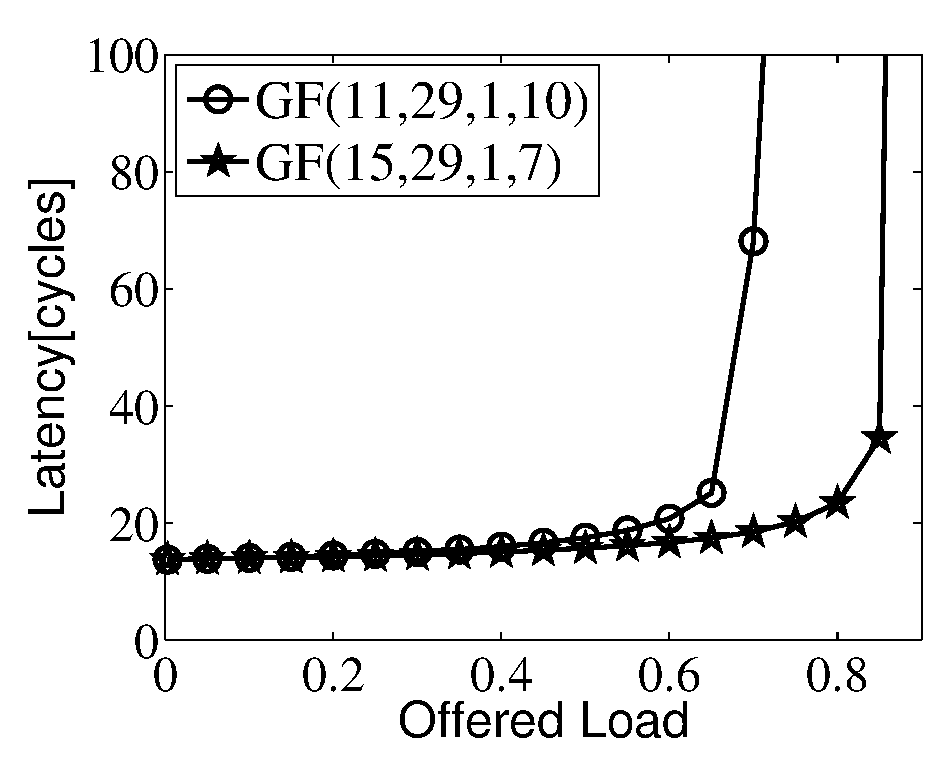
\includegraphics[width=.4\textwidth]{gf_un1.eps}
      \label{gf_un1}
    }
    \subfloat[网络直径$D=3$]{
      \includegraphics[width=.4\textwidth]{gf_ur_b}
      %% 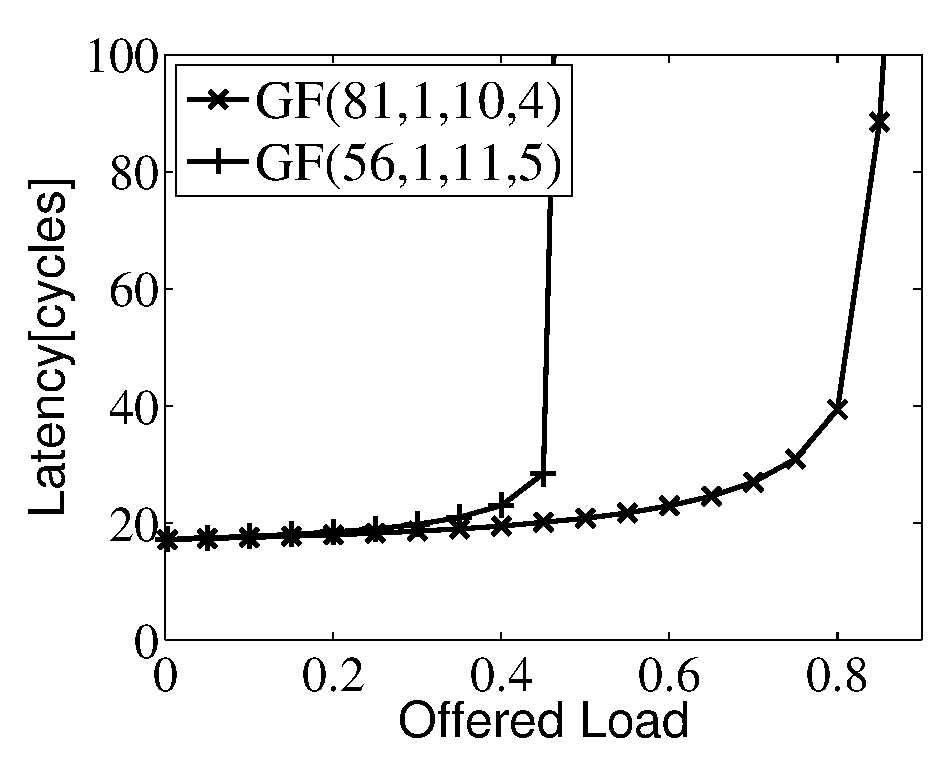
\includegraphics[width=.4\textwidth]{gf_un2.eps}
      \label{gf_un2}
    }
    \\
    \subfloat[网络直径$D=4$]{
      \includegraphics[width=.4\textwidth]{gf_ur_c}
      %% 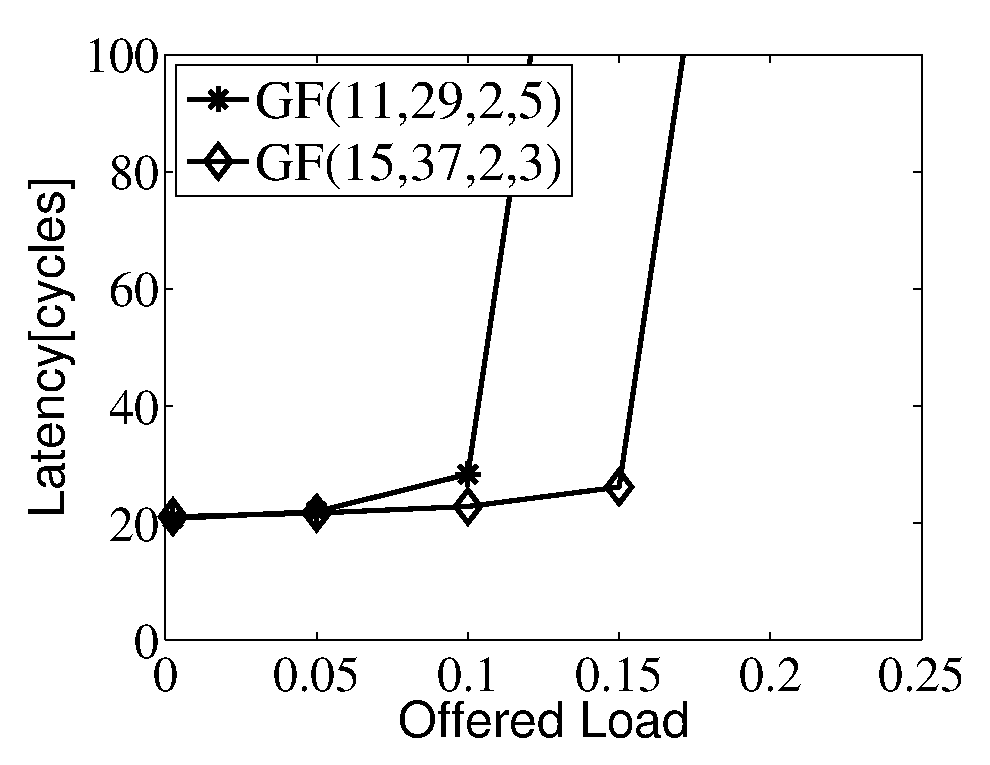
\includegraphics[width=.4\textwidth]{gf_un3.eps}
      \label{gf_un3}
    }
    \subfloat[网络直径$D=5$]{
      \includegraphics[width=.4\textwidth]{gf_ur_d}
      %% 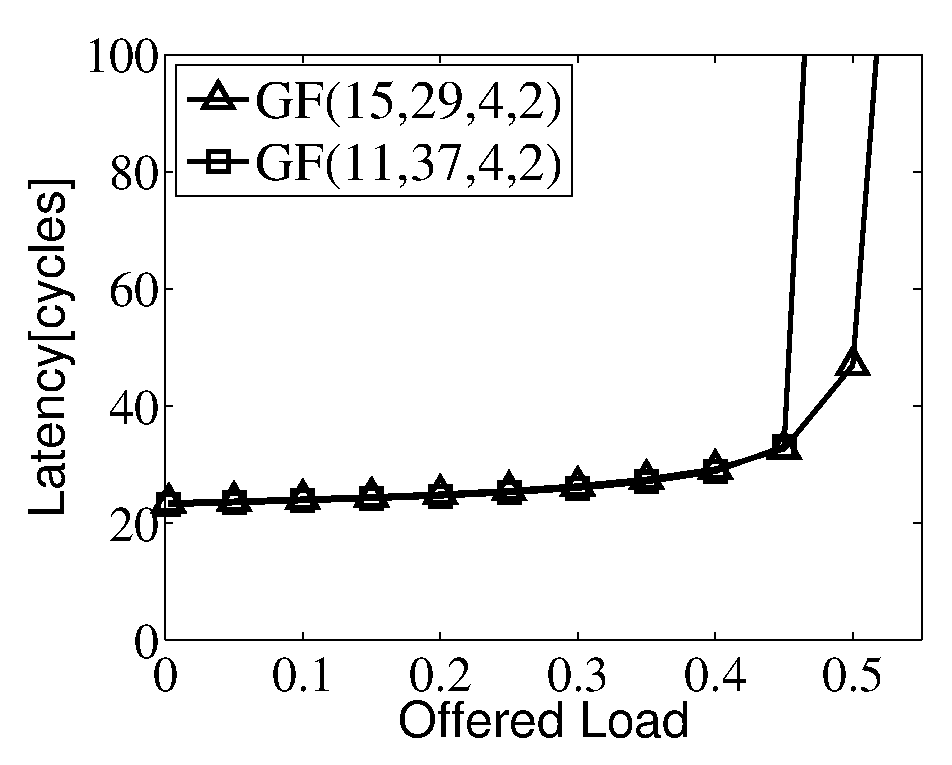
\includegraphics[width=.4\textwidth]{gf_un4.eps}
      \label{gf_un4}
    }
    \caption{不同参数配置下Galaxyfly网络性能(均衡随机通信模式)}
    \label{chap3figure10a}
  \end{minipage}
\end{figure}
\begin{figure}
  \centering
  \begin{minipage}[t]{\textwidth}
    \centering
    \subfloat[网络直径$D=2$]{
      \includegraphics[width=.4\textwidth]{gf_w_a}
      %% 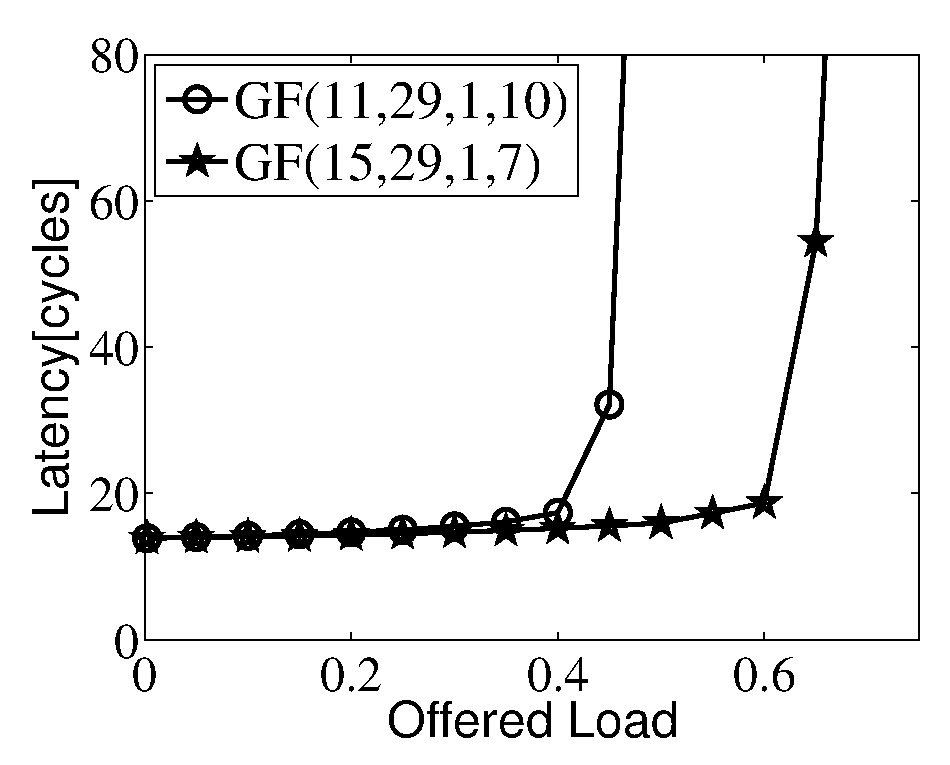
\includegraphics[width=.4\textwidth]{gf_un5.eps}
      \label{gf_un5}
    }
    \subfloat[网络直径$D=3$]{
      \includegraphics[width=.4\textwidth]{gf_w_b}
      %% 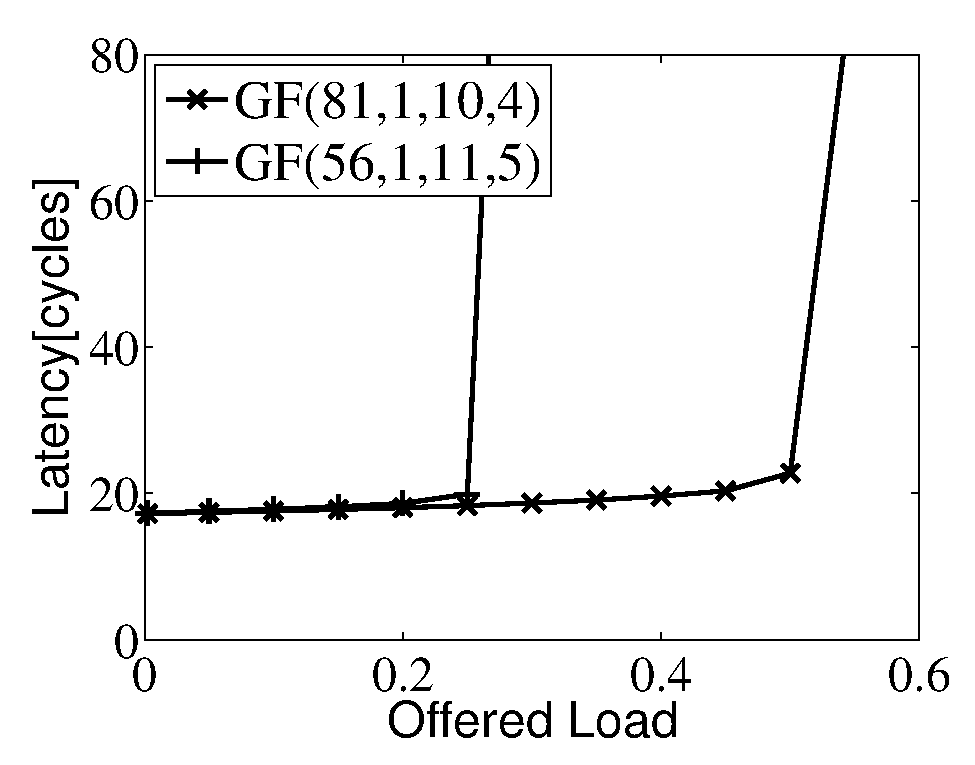
\includegraphics[width=.4\textwidth]{gf_un6.eps}
      \label{gf_un6}
    }
    \\
    \subfloat[网络直径$D=4$]{
      \includegraphics[width=.4\textwidth]{gf_w_c}
      %% 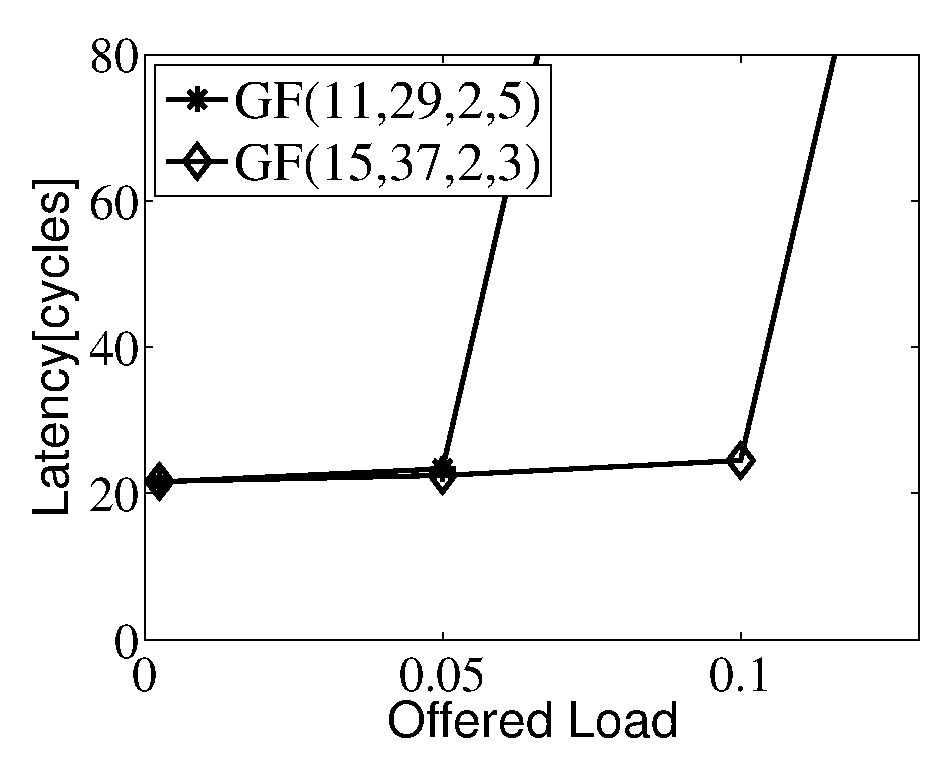
\includegraphics[width=.4\textwidth]{gf_un7.eps}
      \label{gf_un7}
    }
    \subfloat[网络直径$D=5$]{
      \includegraphics[width=.4\textwidth]{gf_w_d}
      %% 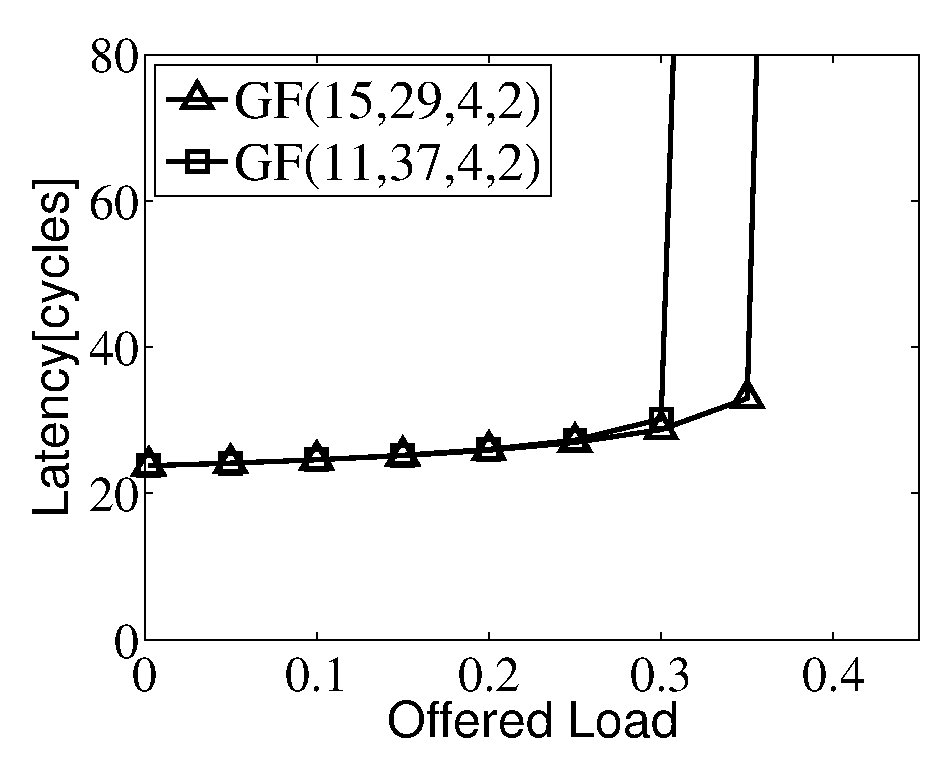
\includegraphics[width=.4\textwidth]{gf_un8.eps}
      \label{gf_un8}
    }
    \caption{不同参数配置下Galaxyfly网络性能(最差通信模式)}
    \label{chap3figure10b}
  \end{minipage}
\end{figure}

我们根据网络直径将表\ref{chap3table6}中列出的不同配置下的Galaxyfly网络划分成组,
比较组内Galaxyfly网络的性能。
图\ref{chap3figure10a}与\ref{chap3figure10b}分别展示了
在均衡随机通信模式与最差通信模式下的性能测试结果。
对照表\ref{chap3table6}可知,
%% GF$(15,29,1,7,28)$、GF$(81,1,10,4,8)$、GF$(15,37,2,3,16)$和GF$(15,29,4,2,7)$的二分带宽
%% 分别高于GF$(11,29,1,10,24)$、GF$(56,1,11,5,5)$、GF$(11,29,2,5,12)$和GF$(11,37,4,2,7)$,
%% 观察图\ref{chap3figure10a}与\ref{chap3figure10b}可知,
无论在均衡随机通信模式或者是最差通信模式下,
网络的二分带宽越高,其饱和吞吐率越高。
以图\ref{gf_un1}和图\ref{gf_un5}为例,
GF$(15,29,1,7,28)$的路由器数量与最小二分切割的链路数分别比
GF$(11,29,1,10,24)$高36.3\%与79.5\%,
在两种通信模式下,GF$(15,29,1,7,28)$的饱和吞吐率比GF$(11,29,1,10,24)$分别高21.5\%和55.6\%。
%% FIXME 这一段分析的insight在那?而且根本没有放在同一张图上
然而,网络直径更短以及二分带宽更高的配置不一定能获得高的饱和吞吐率。
虽然GF$(15,37,2,3,16)$ 的网络直径为4 且$\beta>1$,
在均衡随机通信模式下,GF$(15,37,2,3,16)$的饱和吞吐率为0.15,
仅能达到GF$(11,37,4,2,7)$饱和吞吐率的33\%,
原因在于前者的全局链路数量少于后者。

\subsubsection{报文长度}

我们分析不同的报文长度如何影响Galaxyfly的网络性能。
图\ref{fig:packetsize}展示了不同通信模式下使用不同报文长度的性能测试结果。
由该图可知,在同样配置的Galaxyfly网络中,
报文长度越短,网络延迟越小,但是长报文的饱和吞吐率更高,
对于网络直径较短的Galaxyfly网络尤其如此。
%% FIXME 图要重画,要能高体现出网络直径。
%% 在文字中加上示例。
\begin{figure}
  \centering
  \begin{minipage}[t]{\textwidth}
    \centering
    \subfloat[均衡随机通信模式]{
      \includegraphics[width=.4\textwidth]{packets_a}
      %% \includegraphics[width=.4\textwidth]{lap3.eps}
      \label{lap3}
    }
    \subfloat[最差通信模式]{
      \includegraphics[width=.4\textwidth]{packets_b}
      %% \includegraphics[width=.4\textwidth]{lap4.eps}
      \label{lap4}
    }
    \caption{不同报文长度下Galaxyfly的网络性能}
    \label{fig:packetsize}
  \end{minipage}
\end{figure}

\subsubsection{路由算法}

大规模的高性能计算系统,通信模式更加复杂多样。
我们引进了一种混合通信模式评测路由算法性能,
该混合通信负载包括$90\%$的均衡随机通信模式用于模拟计算节点之间通信,
$10\%$的热点通信模式用于模拟计算节点和固定范围的I/O节点通信。
图\ref{lbr2}展示了GF$(15,29,4,2,7)$在混合通信模式下四种不同路由算法的性能
(其他配置的Galaxyfly也呈现相似的结果)。
NAG算法相比其他路由算法表现出更优的性能。
为定量分析NAG的性能优势,我们分别测试了NAG算法与MIN算法在
不同配置Galaxyfly网络中的性能,结果如图\ref{lbr3}。
在GF$(15,29,1,7,28)$、GF$(15,29,4,2,7)$与GF$(81,1,10,4,8)$网络中,
NAG算法的饱和吞吐率比MIN算法分别高出25\%, 260\%, 与100\%。

\begin{figure}
  \centering
  \begin{minipage}[t]{\textwidth}
    \centering
    \subfloat[GF$(15,29,4,2,7)$]{
      \includegraphics[width=.4\textwidth]{routingalgos_a}
      %% \includegraphics[width=.4\textwidth]{lbr2.eps}
      \label{lbr2}
    }
    \subfloat[MIN与NAG的性能比较]{
      \includegraphics[width=.4\textwidth]{routingalgos_b}
      %% \includegraphics[width=.4\textwidth]{lbr3.eps}
      \label{lbr3}
    }
    \caption{不同路由算法下Galaxyfly的网络性能(混合通信模式)}
    \label{fig:routingalgorithms}
  \end{minipage}
\end{figure}

\subsection{不同拓扑结构的比较}


\subsubsection{与Fat tree的比较}
图\ref{fig:gfft}展示了不同配置的GF与FT的性能对比结果。
在两种通信模式下,GF$(15,29,1,7,28)$与GF$(81,1,10,4,8)$
都表现出比FT更低的网络延迟、更高的饱和吞吐率。
而且,GF$(15,29,1,7,28)$使用的路由器数量仅为FT的64\%。
GF$(15,29,1,7,28)$的性能优于FT有两个原因。
一是网络直径更短,GF$(15,29,1,7,28)$的网络直径为2。
而FT的网络直径更长,同时长路径路由增加了头阻塞的概率。
第二个原因则是较高的全局链路密度,
GF$(15,29,1,7,28)$中每一个路由器80\%的端口用于
%% FIXME 啥意思?
互连同一个集群或者其他集群的其他路由器。
GF$(15,29,4,2,7)$与GF$(81,1,10,4,8)$的路由器数量多于FT,
然而FT必须使用30端口路由器,而它们需要的路由器端口数分别为21与12,
仅为FT路由器端口数的70\%与40\%。
%% FIXME 看不出0负载的东西。
而且,GF$(81,1,10,4,8)$的网络直径为3,在零负载条件下
也优于Fat tree。GF$(15,29,4,2,7)$的网络直径为5,在零负载下略高于Fat tree。

\begin{figure}
  \centering
  \begin{minipage}[t]{\textwidth}
    \centering
    \subfloat[均衡随机通信模式]{
      \includegraphics[width=.4\textwidth]{gfft_a}
      %% \includegraphics[width=.4\textwidth]{df_un1.eps}
      \label{df_un1}
    }
    \subfloat[最差通信模式]{
      \includegraphics[width=.4\textwidth]{gfft_b}
      %% \includegraphics[width=.4\textwidth]{df_un4.eps}
      \label{df_un4}
    }
    \caption{Galaxyfly与FT性能比较}
    \label{fig:gfft}
  \end{minipage}
\end{figure}

\subsubsection{与Flattened Butterfly的比较}
我们也比较了Galaxyfly和Flattened Butterfly的性能差别。
FB是一个高阶的$k-ary$ $n-cube$拓扑结构。
它在每一维上都是一个全互连的网络。
相比FT,FB的路由器数量和链路数更少。
图\ref{fig:gffb}展示了GF和3D FB的性能比较结果。
在均衡随机通信负载下,FB的性能跟GF$(81,1,10,4,8)$的相近,
其主要原因是因为两个网络有相同的网络直径。
虽然FB提供了多于GF$(81,1,10,4,8)$36\%的全局链路
(FB第一维的结构和GF$(81,1,10,4,8)$的超级节点被认为是本地组),
但是FB的全局链路集中在每一维上,而不是分布在整个全局网络上。
另外,在最差通信模式下,FB的饱和吞吐率
与GF$(15,29,4,2,7)$和GF$(81,1,10,4,8)$分别相差62.5\%和70\%。

\begin{figure}
  \centering
  \begin{minipage}[t]{\textwidth}
    \centering
    \subfloat[均衡随机通信模式]{
      \includegraphics[width=.4\textwidth]{gffb_a}
      %% \includegraphics[width=.4\textwidth]{df_un2.eps}
      \label{df_un2}
    }
    \subfloat[最差通信模式]{
      \includegraphics[width=.4\textwidth]{gffb_b}
      %% \includegraphics[width=.4\textwidth]{df_un5.eps}
      \label{df_un5}
    }
    \caption{Galaxyfly与FB性能比较}
    \label{fig:gffb}
  \end{minipage}
\end{figure}

\subsubsection{与Slim Fly和Dragonfly的比较}
图\ref{fig:gfsfdf}展示了不同配置的Galaxyfly与Slim Fly、Dragonfly的性能比较结果。

Slim Fly是最新提出的低直径高阶拓扑结构。
与Galaxyfly相同,Slim Fly也利用了代数图论有限域的方法。
Slim Fly保证网络直径为2,但是,它的低直径属性是基于路由器之间相连的端口数$k'$和路由器
规模$N_r$的最优关系,$k'\geq\Omega(\sqrt N_r)$。
该前提条件严格限制了Slim Fly的扩展性。
相对地,Galayxyfly支持使用固定端口数路由器构造任意规模系统。
GF$(n>1,q>1,a=1,p,h)$,即Galaxy图,也是一个直径为2的拓扑结构,
但在同样网络规模和相近的二分带宽要求下,它比SF需要更高的端口数。
比如,在表\ref{chap3table6}中,GF$(11,29,1,10,8)$
和Slim Fly具有相近的$\beta$,但是GF$(11,29,1,10,8)$的每一个路由器要求
更多的端口数。
GF$(15,29,1,7,28)$是另外一个直径为2的Galaxyfly配置,
具有更高的$\beta$值,也需要更高的路由器端口数。
因此,在Slim Fly和Galaxyfly的多种配置间中的选择,实际上
是性能和路由器端口数的权衡。
在均衡随机通信模式和最差通信模式下,
GF$(15,29,1,7,28)$的饱和吞吐率分别比SF高42\%和140\%。
其主要原因在于它比SF多使用了28\%的路由器和89\%的全局链路。
类似地,GF$(11,29,1,10,24)$在两种通信模式下的饱和吞吐率也分别比SF高8\%和60\%。
GF$(81,1,10,4,8)$是直径为3的网络,其零负载延迟略高于Slim Fly。
但是,在上述两种通信模式下,饱和吞吐率则分别高于SF近33\%和100\%。
而且,GF$(81,1,10,4,8)$的路由器端口数是21,仅为SF的75\%。

%% FIXME 端口数多少?
通常认为,Dragonfly结构是GF$(56,1,11,5)$。
与DF相比,Galaxyfly不仅参数配置更加灵活而且能调整参数获得更好的网络性能。
GF$(81,1,10,4,8)$仅比DF多使用5\%的路由器端口,但是,
其性能在任一通信模式下都能优于DF一倍。
尽管GF$(15,29,4,2,7)$的零负载延迟高于DF,
但在均衡随机通信模式下,GF$(15,29,4,2,7)$可以利用更少得路由器端口获得相似的性能。
而在最差通信模式下,GF$(15,29,4,2,7)$优于DF则是因为在两个集群之间有更多的全局链路。

\begin{figure}
  \centering
  \begin{minipage}[t]{\textwidth}
    \centering
    \subfloat[均衡随机通信模式]{
      \includegraphics[width=.4\textwidth]{gfsfdf_a}
      %% \includegraphics[width=.4\textwidth]{df_un3.eps}
      \label{df_un3}
    }
    \subfloat[最差通信模式]{
      \includegraphics[width=.4\textwidth]{gfsfdf_b}
      %% \includegraphics[width=.4\textwidth]{df_un6.eps}
      \label{df_un6}
    }
    \caption{Galaxyfly与DF,FB性能比较}
    \label{fig:gfsfdf}
  \end{minipage}
\end{figure}

\subsection{物理布局}

Galaxyfly是一个灵活的层次化结构,由多个集群组成。
每一个集群都有同样数目的超级节点,且集群之间的连线数目相同。
Galaxyfly的模块化结构对物理布局有重要意义。
如果超级节点规模很小,那么可以以一个集群为封装单位,即一个集群为一个机柜。
若超级节点规模较大,则可以将一个或多个超级节点封装在一个机柜内。
机柜之间有多条链路,可以通过捆绑的方式连接,
捆绑缆线不仅可以减少缆线成本开销还易于部署\upcite{Jupiter}。
Slim Fly和Dragonfly结构也都是层次化结构,因此它们也可以按照类似于Galaxyfly的思路进行布局。
设置每个机柜都存放200--360个终端,
各网络的物理布局情况如下:
Slim Fly和Dragonfly分别分布在10个和14个机柜内,
GF$(15,29,4,2)$、GF$(15,29,1,7)$ 和GF$(81,1,10,4)$
则分别分布在15、15和9个机柜内。

我们考虑实际物理布局对线缆延迟的影响。
根据物理布局给布局中的本地链路和全局链路赋予不同的延迟值。
机柜内的连线使用电信号,延迟约50个时钟周期。
由于光缆的传输速率和频率,机柜之间的全局链路的平均延迟则设为100个时钟周期。
这里提到的延迟都涵盖了报文穿过路由器模块的延迟。
图\ref{fig:layouts}展示了GF、SF和DF在上述延迟设置下的网络性能。
%% FIXME 这句话啥意思
%% 与前面章节中对所有链路应用相同网络延迟的实验结果相比,
%% 考虑物理布局的实验结果中,网络直径对网络延迟的影响更大。
当比较不同的链路延迟和相同的链路延迟的模拟结果时,
网络直径对不同的链路延迟影响效果大。
因为GF$(15,29,4,2,7)$网络直径最大,其零负载延迟也高于其他拓扑结构。
GF$(15,29,1,7,28)$和GF$(81,1,10,4,8)$的性能都优于SF和DF.
相比于GF$(15,29,1,7,28)$,GF$(81,1,10,4,8)$的饱和吞吐率略高,
主要原因是因为GF$(81,1,10,4,8)$的机柜间链路数量比GF$(15,29,1,7,28)$高59.6\%。
在混合通信模式下,GF$(15,29,1,7,28)$不仅获得最高的饱和吞吐率而且网络延迟最低。
DF和GF$(81,1,10,4)$在注入率0.25和0.35附近延迟突然增加,
出现这种现象的原因是路由算法在该点由最短路径路由切换到非最短路径路由。

\begin{figure}[t]
  \centering
  \begin{minipage}[t]{\textwidth}
    \centering
    \subfloat[均衡随机通信模式]{
      \includegraphics[width=.31\textwidth]{layouts_a}
      %% \includegraphics[width=.31\textwidth]{lap1.eps}
      \label{lap1}
    }
    \subfloat[最差通信模式]{
      \includegraphics[width=.31\textwidth]{layouts_b}
      %% \includegraphics[width=.31\textwidth]{lap2.eps}
      \label{lap2}
    }
    \subfloat[混合通信模式]{
      \includegraphics[width=.31\textwidth]{layouts_c}
      %% \includegraphics[width=.31\textwidth]{lbr1.eps}
      \label{lbr1}
    }
    \caption{实际物理布局下GF,SF与DF的网络性能比较}
    \label{fig:layouts}
  \end{minipage}
\end{figure}

\section{成本和功耗开销}
本节讨论Galaxyfly和其他拓扑结构构建网络的两个主要成本:
(1)路由器和缆线的成本开销与(2)功耗开销。

高性能计算机系统中,所有计算节点、路由节点以及缆线
在实际部署时被部署在一个2维的矩形框架中。
系统部署关注的一个主要问题是如何使用尽量少的链路开销完成互连网络的布线。
一个好的拓扑结构可以大大提升系统物理部署中的布线效果。
Galaxyfly的层次化结构非常适合划分成若干个模块。每一个机柜内都部署
一定数量的路由器及其连接的终端并使得机柜之间的链路数基本相等。
Galaxyfly可以按集群或者超级节点划分模块。
因此,可以通过控制参数$(n,q,a,p,h)$之间的关系来控制整个Galaxyfly网络的成本开销。

\subsection{成本分析}

我们引进一个与文献\upcite{slimfly}和文献\upcite{Flattenedbutterfly}
类似的成本模型来分析整个互连网络的成本开销。
互连网络的主要开销集中在路由器和缆线上。
假设路由器和终端被封装在一个$1 \times 1 \times 2$米的机柜中。
机柜内使用电缆,而机柜间则使用光缆。
为了计算缆线的长度,保守假设机柜内的缆线的平均长度约为1--1.5米,
机柜间的缆线长度则使用3维立方体的曼哈顿距离估算得到\upcite{slimfly},
每一条机柜间缆线的距离还要额外加上2米的机柜内的开销。

%% FIXME 这句话解释一下

我们比较了Galaxyfly、Dragonfly、Regular Random结构(RR)\upcite{acaserandom}、
3维Flattened Butterfly、3层Fat tree和Slim Fly的成本开销。
各个拓扑结构均采用负载均衡配置,网络规模$N\approx30K$,且差别范围控制在1--3\%。
%% 在确定机柜数为$c$的情况下,
为了均衡缆线长度,所有网络中的机柜都被布局到一个$x\times y+z$的矩形框中。
我们分析缆线开销时为不同的拓扑结构设计了合适的布局方式,
使得每个机柜封装规模相近的终端,如对于Dragonfly,一个机柜封装一个超级节点。
具体来说,Dragonfly、Fat tree、Flattened Butterfly、Slim Fly、Regular Random结构
和5个不同配置的Galaxyfly分别被封装在
$13\times13+3$、 $9\times16+12$、$13\times13$、
$13\times12+6$、$13\times13+3$ 和$13\times13+7$的矩阵中。

为了评估每个拓扑的成本开销,我们使用了缆线和路由器的实际价格\upcite{colf}\upcite{mella},
线缆和路由器的价格走势分别如图\ref{crp1}和图\ref{crp2}所示。
各个拓扑结构的缆线开销如图\ref{crp3}所示。
Fat tree的布局不同于其他拓扑结构,因为其是间接拓扑,
%% FIXME 是7还是9?
所以叶子路由器和终端被封装在$7\times 16+12$的机柜中,
并且不得不考虑叶子路由器和终端之间的连接关系。
由于层次间的大量连线,Fat tree的光纤开销是所有拓扑结构最高的。
Regular Random结构的路由器端口数和物理布局都跟Dragonfly的一样,
但是大量机柜间的链路使得Regular Random结构的链路开销高于其他直接拓扑结构。
5个不同配置的Galaxyfly详细参数如表\ref{chap3table7}所示。
这5个Galaxyfly采用相同的物理布局,因此机柜间光缆开销相同。
这五个Galaxyfly缆线开销的区别在于机柜内部的链路开销。
GF$(25,49,1,24,48)$是性价比最高的结构,他的缆线开销比Slim Fly还要低5\%。

\begin{figure}
  \centering
  \begin{minipage}[t]{\textwidth}
   \centering
  \subfloat[线缆价格]{
  \includegraphics[width=.4\textwidth,height=.32\textwidth]{crp1.eps}
  \label{crp1}
  }
  \subfloat[路由器价格]{
  \includegraphics[width=.4\textwidth,height=.32\textwidth]{crp2.eps}
  \label{crp2}
  }
  \caption{成本开销模型}
  \label{fig:Figure15}
  \end{minipage}
\end{figure}
\begin{figure}
  \centering
  \includegraphics[width=.6\textwidth,height=.32\textwidth]{crp3.eps}
  \caption{不同网络的线缆成本}
  \label{crp3}
\end{figure}

%% FIXME 这里用到的GF配置完全不同于前面的。
表\ref{chap3table7}列出了不同拓扑结构的路由器成本开销。
GF$(25,49,1,24,48)$需要的路由器端口数是所有拓扑结构中最大的。
但是,GF$(25,49,1,24)$结构是性价比最高的拓扑结构,
而Dragonfly、Fat tree、Flattened Butterfly 以及Slim Fly的路由器开销分别比
GF$(25,49,1,24,48)$高36.8\%、68.4\%、27.1\%和2.2\%。
尽管GF$(25,49,8,3,6)$是性价比最低的拓扑结构,但是,
GF$(25,49,8,3,6)$需要的路由器端口数最少,只有Dragonfly的$44\%$,Fat tree
的$25.8\%$,Flattened Butterfly的$32.7\%$,Slim Fly 的$26.2\%$。
%% 另外,能够调整Galaxyfly的参数满足路由器开销和路由器端口数的要求。
通过调整超级节点的规模$a$,GF$(25,49,3,8,16)$、
GF$(25,49,4,6,12)$ 和GF$(25,49,6,4,8)$能获得比GF$(25,49,8,3,6)$
更低的路由器成本开销,而且路由器端口数需求也小于其他拓扑结构。


\begin{table}[t]
\centering
\caption{不同网络的路由器成本和功耗}
\begin{tabular}{cccccc}
  \toprule
  Topology & $N$ & $N_r$ & $r$ & 路由器成本/终端(美元) & 功耗/终端(W)\\
  \midrule
  DF & 29412 & 3268 & 36 & 1130 & 21 \\
  FT & 29791 & 2883 &62 & 1391 & 24\\
  FB & 28561 & 2197 &49 &1050 &21 \\	
  SF & 29160 &1458 & 61 & 844 & 19\\	
  GF$(25,49,8,3,6)$ &29400 &9800 &16 &1602 &25 \\
  GF$(25,49,3,8,16)$ &29400 &3675 &26 &936 &19 \\
  GF$(25,49,4,6,12)$ &29400 &4900 &21 &1025 &20 \\
  GF$(25,49,6,4,8)$ &29400 &7350 &17 &1269 &22 \\
  GF$(25,49,1,24,48)$ &29400 &1225 &72 &826 &18 \\
  \bottomrule
\end{tabular}
 \label{chap3table7}
\end{table}

%% 我们也可以划分结构以Galaxyfly 的集群为单位。在不同的物理布局下,
%% 不同拓扑结构的缆线开销趋势一致。Galaxyfly在合适的配置下可以
%% 构造出性价比高的结构。

\subsection{功耗分析}

互连网络的功耗在整个高性能计算机系统中功耗占比可高达50\%\upcite{Energy}。
我们采用功耗模型如下:路由器每个端口4个SerDes且每个端口的功耗约为2.8瓦特,
每个计算节点的网口控制器工作功耗为10瓦特。

表\ref{chap3table7}展示了Galaxyfly和其他拓扑结构在该功耗模型下的开销。
从表中可以看出,功耗成本基本和路由器数量成正比。
GF$(25,49,1,24,48)$是功耗开销最小的网络,因为它使用了最少的路由器。

\section{本章小结}

高阶拓扑结构是当前和未来大规模高性能计算系统互连网络采用的主流拓扑结构。
但是,高阶路由器端口数的增长受限于当前SerDes面积、Crossbar仲裁以及功耗
开销等因素。本章提出了一个新型低直径高阶拓扑结构,Galaxyfly。
它不仅具备很强的规模灵活性,支持构建从P级系统到E级系统甚至更大规模的计算系统,
同时还可以有效降低对路由器端口数的需求。
Galaxyfly拓扑结构可以通过参数配置在网络性能、物理布局复杂度和成本功耗开销
等因素之间做灵活折中。
